\documentclass{ctexart}
\usepackage{xcolor}
\usepackage{setspace}
\usepackage{tikz}
\usepackage{ctex}
\usepackage{geometry}
\usepackage{amsmath}
\usepackage{graphicx} 
\usepackage{subfigure}
\usepackage{float}
\usepackage{algorithm}  
\usepackage{algorithmicx}  
\usepackage{algpseudocode} 
\usepackage{url}
\usepackage{amsthm, amssymb, appendix, bm, graphicx, hyperref, mathrsfs}
\usepackage{tabularx}
\usepackage{booktabs} %需要加载宏包{booktabs}
\usepackage{multirow}
\usepackage{diagbox} % 加载宏包
\usepackage{pifont}

\usepackage{siunitx}
\usepackage{listings}
\usepackage{float}
\pagestyle{plain}

\usetikzlibrary{datavisualization}
\usetikzlibrary{arrows,shapes,chains}
\usepackage{listings}
\lstset{language=C++}
\lstset{breaklines}
\lstset{extendedchars=false}
\lstset{numbers=left}
\geometry{a4paper,left=2.5cm,right=2.5cm,top=2.5cm,bottom=2.5cm}
\CTEXsetup[format={\Large\bfseries\centering}]{section}
\tikzstyle{startstop} = [rectangle,rounded corners, minimum width=3cm,minimum height=1cm,text centered, text width=6cm,draw=black]
\tikzstyle{io} = [trapezium, trapezium left angle = 70,trapezium right angle=110,minimum width=5cm,minimum height=1cm,text centered,draw=black,fill=white]
\tikzstyle{process} = [rectangle,minimum width=3cm,minimum height=1cm,text centered,text width =3cm,text width=6cm,draw=black]
\tikzstyle{decision} = [diamond,minimum width=3cm,minimum height=1cm,text centered,text width=6cm,aspect=2,draw=black,thin]
\tikzstyle{arrow} = [thick,->,>=stealth]
\renewcommand{\algorithmicrequire}{\textbf{Input:}}  % Use Input in the format of Algorithm  
\renewcommand{\algorithmicensure}{\textbf{Output:}} % Use Output in the format of Algorithm  
\newcommand{\subsubsubsection}[1]{\paragraph{#1}\mbox{}\\}
\setcounter{secnumdepth}{4} % how many sectioning levels to assign numbers to
\setcounter{tocdepth}{4} % how many sectioning levels to show in ToC
\begin{document}
\begin{spacing}{2.0}
  \begin{center}
      {\LARGE\textbf{基于投票机制及二分法的纯方位无源定位研究}}\\
      {\Large\textbf{摘要}}\\
  \end{center}
\end{spacing}

本文研究的是集群无人机的纯方位无源定位方式,通过建立投票机制模型及二分移动路径法求解得到接收信号无人机的真实位置,从而对其进行调整。

整体问题从已知所有无偏差发射信号无人机的方向信息,到缺失一架发射信号无人机的编号信息,再到所有发射信号无人机均有偏差且编号未知,问题所给信息量逐渐减小。从少量信息中提取有效信息实现定位是本问题的关键所在。

\textbf{针对问题一:}\quad 本题需要在已知3架无偏无人机给出的方向信息的情况下,给出接收端无人机的具体定位。将无人机抽象为四个点进行平面几何分析,发现随着接收端无人机相对其余三个点的位置发生改变,定位计算公式也会随之改变。因此我们用$FY00$与其余两个发射源之间的连线将平面划分成\textbf{四个区域},得到四个不同的计算公式。由于接收端无人机落在哪个区域初识是未知的,故可以通过方向信息计算出4个解。同时因为接收端无人机的位置偏移是略微的,故我们采用距离其标准位置最近的点为其真实位置。为检验模型的准确性,我们模拟了100000次随机的有偏移的初始位置,发现在\textbf{偏移误差小于30\%}的情况下,定位的准确性均可达到\textbf{100\%},说明模型效果良好。进一步扩大误差后,我们发现选取\textbf{圆心角为40$^{\circ}$的两个发射源}相较其余三种(80$^{\circ}$,120$^{\circ}$,160$^{\circ}$)定位错误率更低。

\textbf{针对问题二:}\quad 题目要求利用若干编号未知的发射信号无人机实现定位。为了利用问题一中模型,考虑先确定发射信号无人机的编号,
再调用问题一中模型求解。

首先我们尝试直接\textbf{线性划分}不同角度的信号、对应
不同的信号来源无人机,建立了简单模型。
由于精度不高,我们考虑待定位无人机在以理想位置为圆心的\textbf{误差圆}内随机游动,改变误差圆半径、计算不同半径下各可能信号源无人机
形成的圆周角范围,再累积测得的真实角度落在各个信号源的角度范围的频次。通过上述\textbf{投票机制},选择出最可能的信号源编号。接着我们代入此编号无人机
求解对应的圆周角进行\textbf{角度验证},若与测得的角度偏差超过限度,则认为编号确定错误。从而再引入一架发射信号的无人机,重复上述过程投票选出一对无人机
编号组合,计算得到真实位置。

在模拟1000000次初始情况后,我们发现在\textbf{$20\%$}的偏移误差下,投票机制模型能达到100\%的正确性,而在\textbf{$40\%$}的偏移误差下,仍有\textbf{7\%}的错误率,而再引入一架无人机后,该错误率能降至\textbf{2\%},符合有效定位的要求。
\textbf{针对问题三:}\quad 本题需要将圆周上与标准位置有所偏差的9架无人机调整到尽可能接近标准位置。我们将$FY01$设为基准无人机,使用\textbf{二分移动路径法}确定待测无人机和坐标原点的相对方向,再通过解三角形得到所有待测无人机到原点的距离,最后再用一轮指令调整至标准位置。对于题目给出的初始情况,我们使用\textbf{253次}发射信号或移动操作将所有无人机调整到理想位置附近,所有无人机的偏差距离和仅为\textbf{$0.000160328m$}。我们还自行随机生成了$10^6$组不同的初始情况,根据我们的模型得出的方案进行调整,最终偏差距离和均\textbf{小于$10^{-3}m$}。

\textbf{针对问题四:}\quad 本题将调整其他无人机编队队形中的无人机至标准位置,以题目中所给的锥形无人机编队图为例,我们考虑应用类似问题三的解决思路,我们将$FY01$设为坐标原点,将$FY05$设为基准无人机,使用类似的\textbf{二分移动路径法}和解三角形方法定位所有待测无人机位置,最后用一轮指令调整至标准位置。我们可以用$20$轮询问和调整将每个无人机的角度偏差降低到$10^{-5}$弧度之内。


\quad

\textbf{关键词: \quad 无源定位 \quad 误差圆 \quad 多伦投票机制\quad 二分移动路径法 }

\newpage
\section{问题的背景与重述}
\subsection{问题的背景}
随着无人机制造技术的不断进展,无人机已经被广泛地运用到军事、物流、探测等多个领域,越来越多地进入国家生活的方方面面。而在与无人机相关的工程技术中,如何控制无人机机群保持一定的队形编队飞行,更是现在无人机技术大规模应用的重点与难点。在相关的控制方法研究中,利用无人机间相互信号收发定位的纯方位无源定位方法,以其抗干扰能力强、信号传输隐蔽、能很好适应不同的环境[1],而成为无人机编队飞行的一种良好解决方案。因此探究在纯方位无源定位方法下,无人机编队定位与队形调整的数学模型与算法实现具有重要的研究价值。

\subsection{问题的重述}
根据题目要求,本文旨在解决下列问题:

(1)在圆形飞行编队中,利用圆心处的FY00和两架圆周上已知编号的无人机发射信号,尝试建立接收信号无人机的定位模型。

(2)在圆形飞行编队中,利用FY00、FY01以及若干圆周上未知编号的无人机发射信号,建立接收信号无人机的定位模型。

(3)仍在圆形飞行编队中,每次选择FY00和圆周上最多3架无人机遂行发射信号,依此确定调整方案使得多次调整后机群最终均匀分布在某个圆周上。

(4)转为考虑在锥形飞行编队中,类似三题一般地确定信号发射方案与队形调整方案,使得多次调整后机群队形变为所要求的锥形队列。

\section{问题分析}
\textbf{对于问题一:}问题一要求在发射信号的无人机位置无偏差且编号已知的情况下,对被动接收信号的无人机进行定位。将3架已知无人机(A、B、C)与1架未知无人机(D)的位置抽象化,对其几何图形进行分析。根据AB、AC的连线将整个平面分成区域,D点落在不同的区域即有不同的位置计算公式。由于在实际情况中,D点所在的区域是未知的,4个解均有可能,故我们选用离D点标准位置最近的点作为其真实位置。同时我们进一步探究了已知发射源的选取位置优劣性。

\textbf{对于问题二:}题目要求利用若干编号未知的发射信号无人机实现定位。首先我们利用不同信号源无人机与待定位无人机形成的圆周角不尽相同,直接对角度进行线性划分确定信号源。

进一步我们考虑待定位无人机位置的误差圆,对不同半径下的可能信号源进行统计,综合选出最可能的信号源编号。接着我们代入此编号无人机求解对应圆周角进行验证,若与测得的角度偏差超过限度,则认为编号确定错误。此时我们类似地再引入一架发射信号的无人机,进行下一轮投票,直至符合误差。

\textbf{对于问题三:}选取$FY00$作为坐标原点,$FY01$作为基准无人机,通过二分法多次调整并发射信号测试ℹ,判断其他圆周上的无人机的方向,再通过解三角形得到其到坐标原点的距离。最后通过已确定位置的$FY02$和相关角度信息计算$FY01$的方向和距离,并一次调整令所有圆周上的无人机移动到标准位置附近。
    
\textbf{对于问题四:}选取$FY01$作为坐标原点,$FY05$作为基准无人机,用和问题三类似的方法确定除了$FY05$和$FY13$的位置信息,最后通过已确定位置的$FY02$和相关角度信息计算$FY05$和$FY13$的方向和距离,并全部调整到理想位置附近。


\section{模型假设}
1. \quad 基于自身感知的高度信息,本文默认无人机均保持在同一个高度上飞行,即所有无人机在同一个平面上。

2. \quad 假设第一问中的所有小问9架无人机理论上都应均匀分布在半径为100m的圆周上。

3. \quad 假设无人机接收到的方向信息不存在误差。

4. \quad 本题均拟采用纯方位无源定位的方法调整无人机的位置。

5. \quad 假设当没有调整指令时,无人机编队中的每架飞机都在向相同方向以相同速度前进,即编队整体在向某个方向移动。

6. \quad 假设无人机在调整位置时获得的是(x,y)型指令。

\section{符号说明}

\begin{table}[H]
  \centering
  \begin{tabular}{ccc}
  \toprule
  符号& 含义& 单位\\
  \midrule
  O&FY00编号无人机所在点&/\\
  P&FY01编号无人机的所在点&/\\
  F&可能发射源&/\\
  $F_{truei}$&真实的第i个发射源&/\\
  J&接收点的真实位置&/\\
  Q&误差圆编号(按半径依次编号)&/\\
  I&误差圆的圆心编号&/\\
  $(O_{min},O_{max})$&包含O点的角度范围&$^{\circ}$\\
  $(P_{min},P_{max})$&包含O点的角度范围&$^{\circ}$\\
  $vote_F$&发射源得票数&/\\
  FYi&FY0i编号无人机的理想位置&/\\
  $FYi^{'}$&FY0i编号无人机的真实位置&/\\
  $FYi^{''}$&FY0i编号无人机二分调整后的位置&/\\
  $(\Delta X_{i,j},\Delta Y_{i,j})$&第i次第j号无人机的移动指令&m\\
  \bottomrule
  \end{tabular}
  %\caption{这是一张三线表}\label{tab:aStrangeTable}  标题放在这里也是可以的
  \end{table}




\section{模型的建立与求解}

\subsection{问题一模型的建立与求解}

\subsubsection{极坐标系的建立}

为了更加明确地标注出各编号无人机的标准位置,我们选用包含角度信息的极坐标系来进行刻画。由于被动接收信号的无人机仅能接收到方向信息,即角度,故极坐标系相比直角坐标系更易表达清晰。

假设9架无人机(编号FY01$\sim$FY09)均匀分布在一个半径为100m的圆周上。以编号FY00的无人机作为坐标原点,编号FY00与编号FY01之间的连线作为X轴,建立极坐标系如下图\ref{极坐标系示意图}。各个编号的标准坐标信息如下表:

\begin{figure}[H]
  \centering
  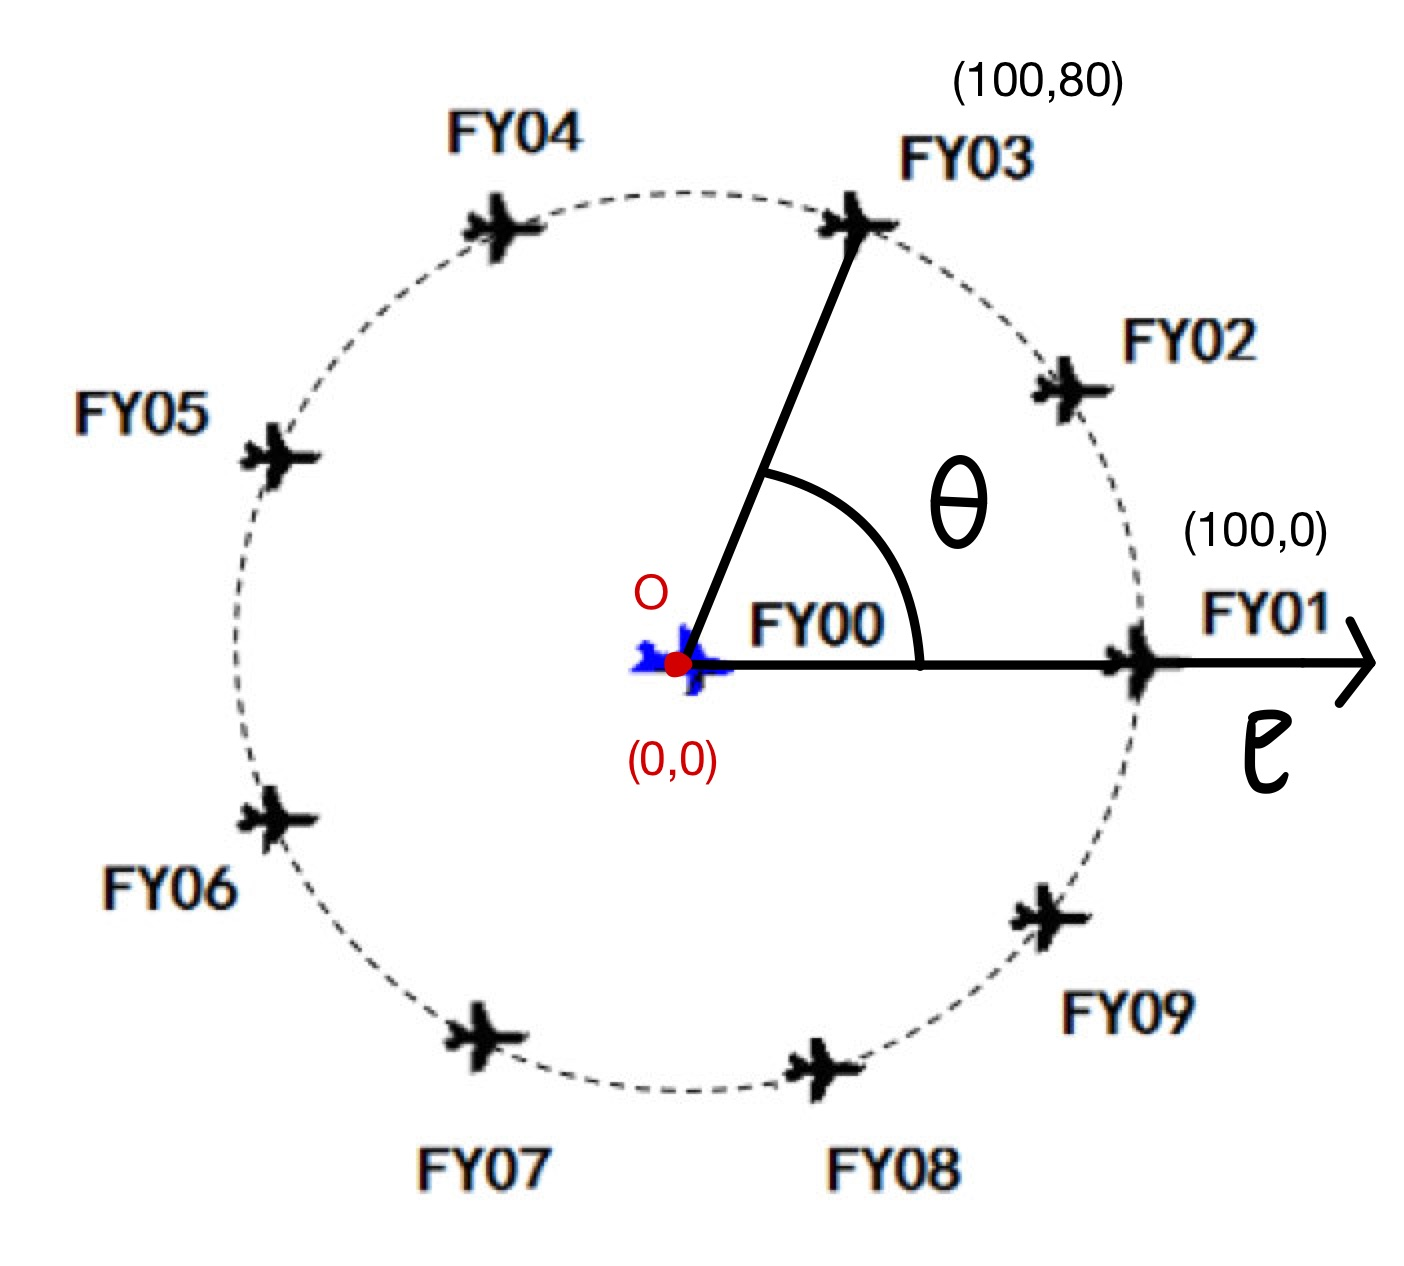
\includegraphics[width=0.40\linewidth]{pic/极坐标.jpg}
  \caption{极坐标系示意图}
  \label{极坐标系示意图}
  \end{figure} 

\begin{center}
  表1:各编号无人机标准坐标
  ~\\
    \begin{tabular}{|c|c|c|c|c|c|}
        \hline
        无人机编号&极坐标(m,$^{\circ}$)&无人机编号&极坐标(m,$^{\circ}$)&无人机编号&极坐标(m,$^{\circ}$)\\
        \hline
        FY00&(0,0)&FY01&(100,0)&FY02&(100,40)\\
        \hline
        FY03&(100,80)&FY04&(100,120)&FY05&(100,160)\\
        \hline
        FY06&(100,200)&FY07&(100,240)&FY08&(100,280)\\
        \hline
        FY09&(100,320)& & & &\\    

        \hline
    \end{tabular}\\
\end{center}
\subsubsection{定位模型的建立}
题目要求在已知未知定位无人机与任意两架发射源无人机间连线的夹角后,给出未知定位无人机当前的所在位置。由于发射源无人机的位置是无偏差的,故它们间的距离同样为已知信息。对该问题进行几何分析:

图中A、B、C三点为已知位置的发射源无人机(A为原点,B、C点在圆上按逆时针顺序排列),三点将平面区域划分为4各部分。D点为需要求解的无人机的位置,可能落在任意一个区域中。如下图\ref{区域划分示意图}所示:

\begin{figure}[H]
  \centering
  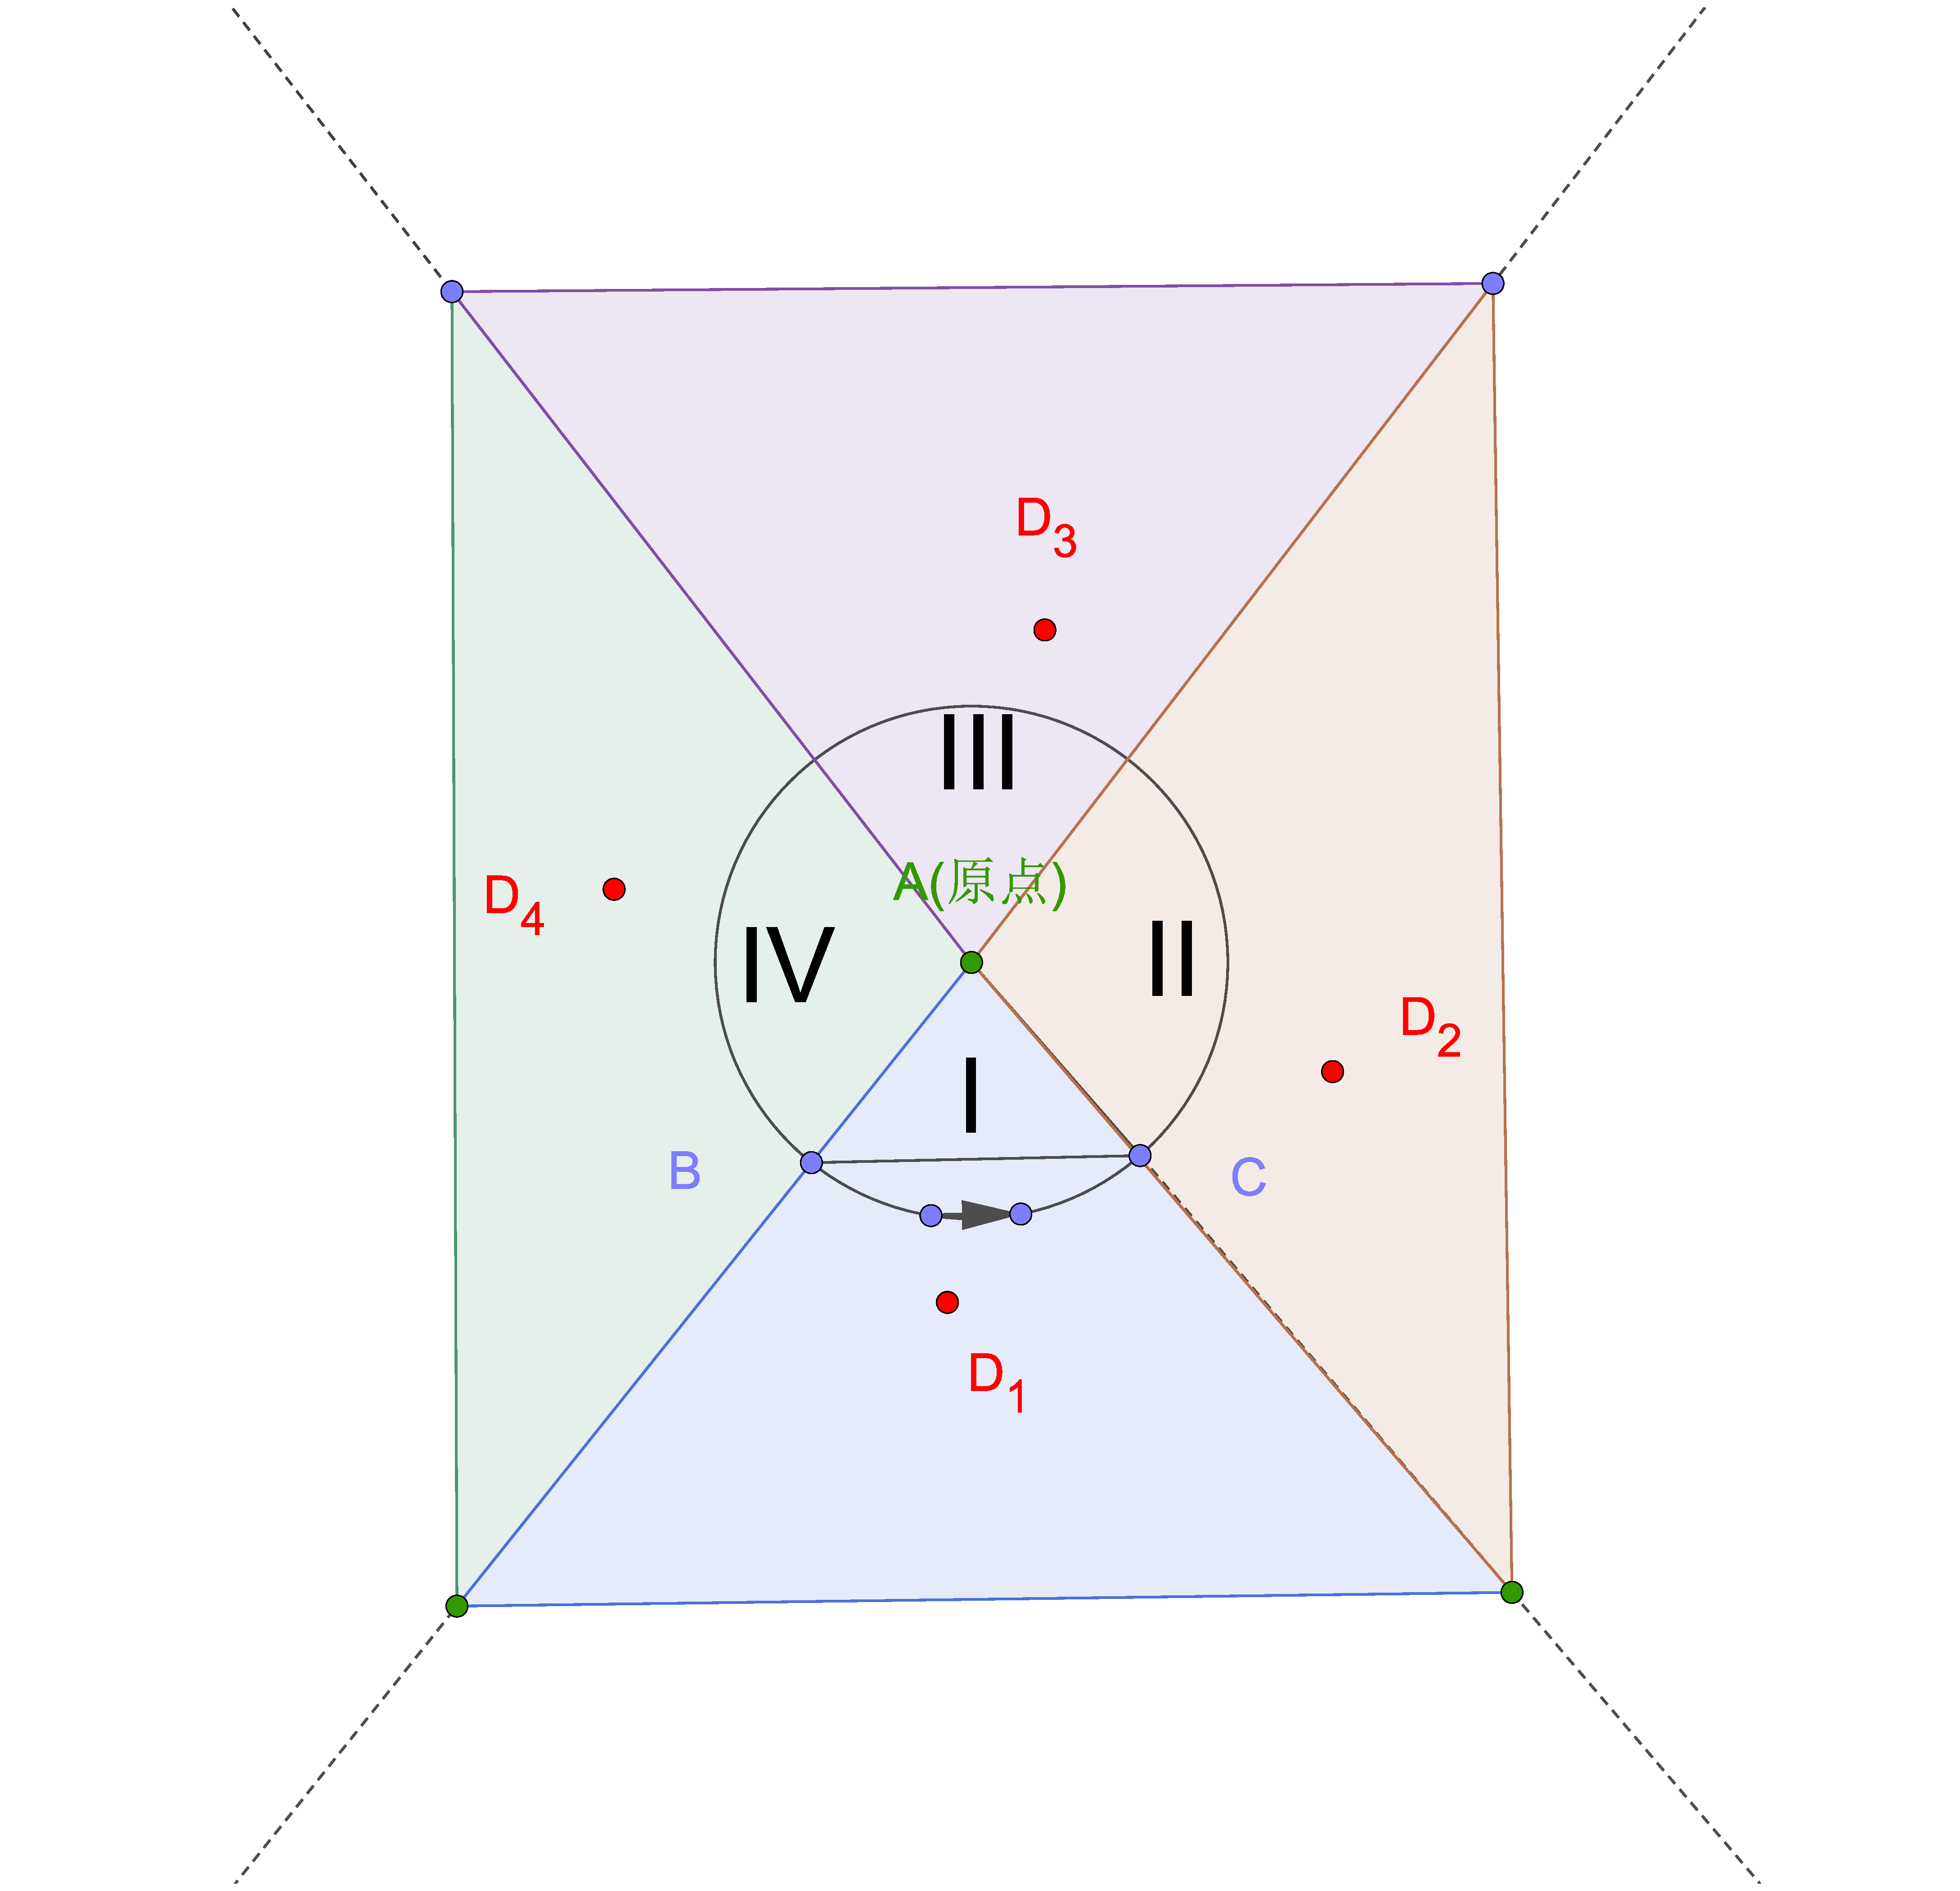
\includegraphics[width=0.40\linewidth]{pic/quadrant(1).eps}
  \caption{区域划分示意图}
  \label{区域划分示意图}
  \end{figure} 


其中,A、B和A、C间的距离均为半径r。已知的方向信息包含两个小角与小角组合形成的大角,实际有效信息仅含两个角度。为了方便计算,我们选择包含原点A的角度$\alpha_1$、$\alpha_2$以及发射源无人机间的夹角$\alpha_3$进行分析。

对每个部分的点分别建立定位模型如下:

利用正弦定理及角度关系对$\Delta$ABD,$\Delta$ACD,$\Delta$BCD进行分析,分别列出下列等式:

设$\angle ABD=\theta_1$,$\angle ACD=\theta_2$,$\angle ADB=\alpha_1$,$\angle ADC=\alpha_2$,$\angle BAC=\alpha_3$,AD=l。

(1)若$\alpha_1$、$\alpha_2$之间不存在包含关系,即D点落在I、III区域,分为两种情况讨论:

若D点落在I区域,如图\ref{区域I典型图},则:

\begin{figure}[H]
  \centering
  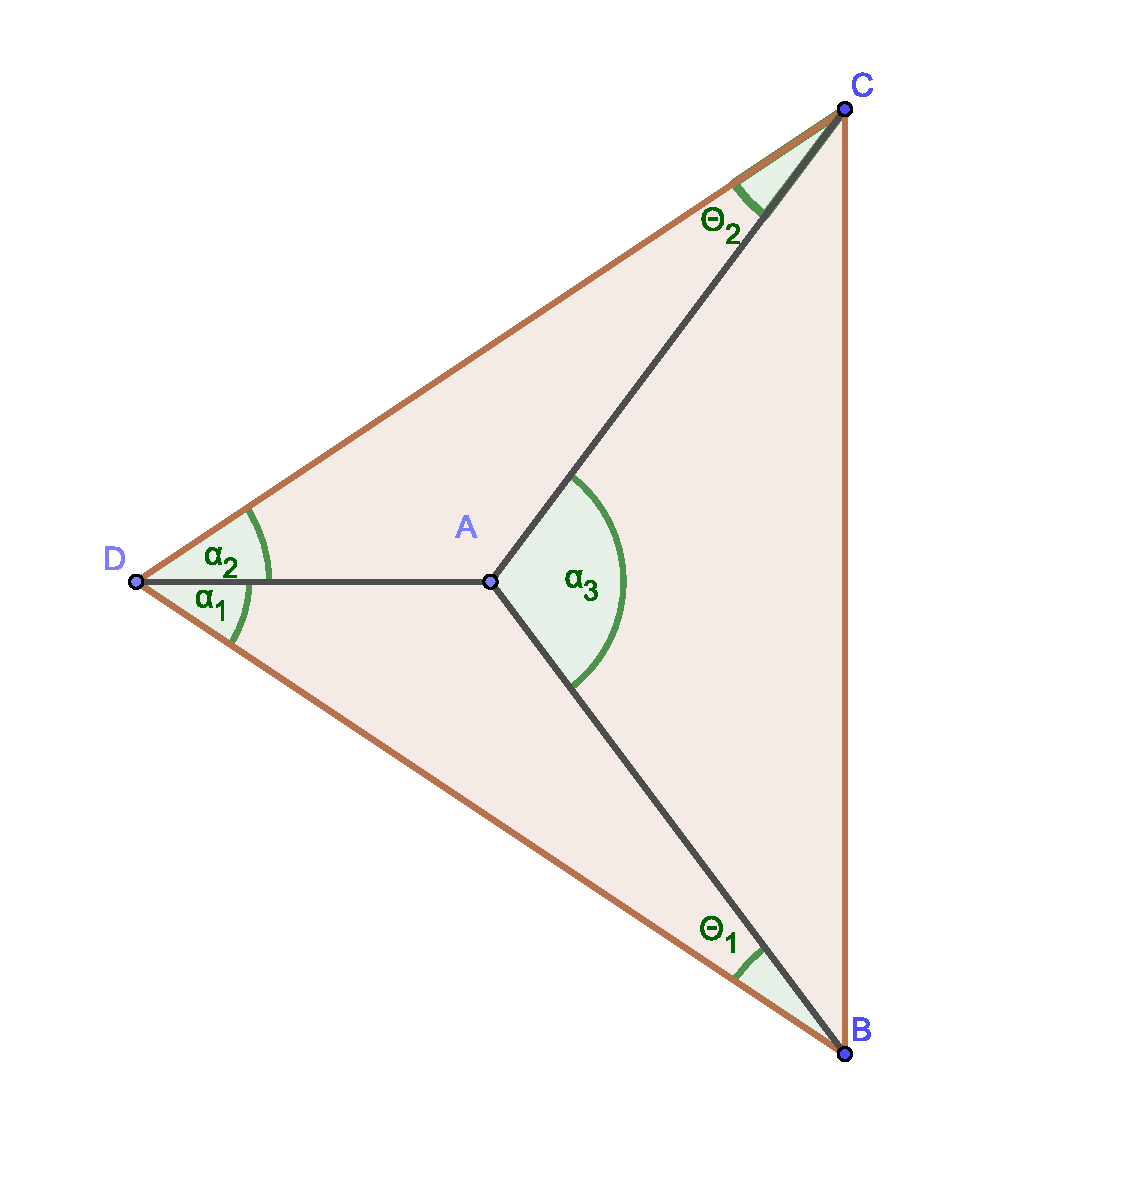
\includegraphics[width=0.35\linewidth]{pic/case1++.eps}
  \caption{区域I典型图}
  \label{区域I典型图}
  \end{figure} 

\begin{equation}
    \left\{
              \begin{array}{ll}
                \theta_1+\theta_2=\alpha_3-(\alpha_1+\alpha_2)=\theta_0\\
                \frac{sin\theta_1}{l}=\frac{sin\alpha_1}{r}=k_1\\
                \frac{sin\theta_2}{l}=\frac{sin\alpha_2}{r}=k_2\\

              \end{array}
            \right.
\end{equation}

\[
    \Rightarrow sin(\theta_0-\theta_1)=\frac{k_2}{k_1}sin\theta_1
\]
\[
    \Rightarrow sin\theta_0 \cdot cos\theta_1-cos\theta_0 \cdot sin\theta_1=\frac{k_2}{k_1}sin\theta_1
\]

\[
    \Rightarrow \theta_1=arctan(\frac{sin\theta_0}{\frac{sin\alpha_2}{sin\alpha_1}+cos\theta_0}),\theta_0=\alpha_3-(\alpha_1+\alpha_2)
\]

在求解过程中,如果发现等式无法计算或出现正无穷的情况,则考虑$\theta_1=90^{\circ}$。

若B的极坐标为(100,$\beta$),则该种情况下,未知点的定位坐标为(100$\times\frac{sin\theta_1}{sin\alpha_1}$,$\beta -$($\pi$-$\theta_1$-$\alpha_1$))。



若D点落在III区域,如图\ref{区域III典型图},则:

\begin{figure}[H]
  \centering
  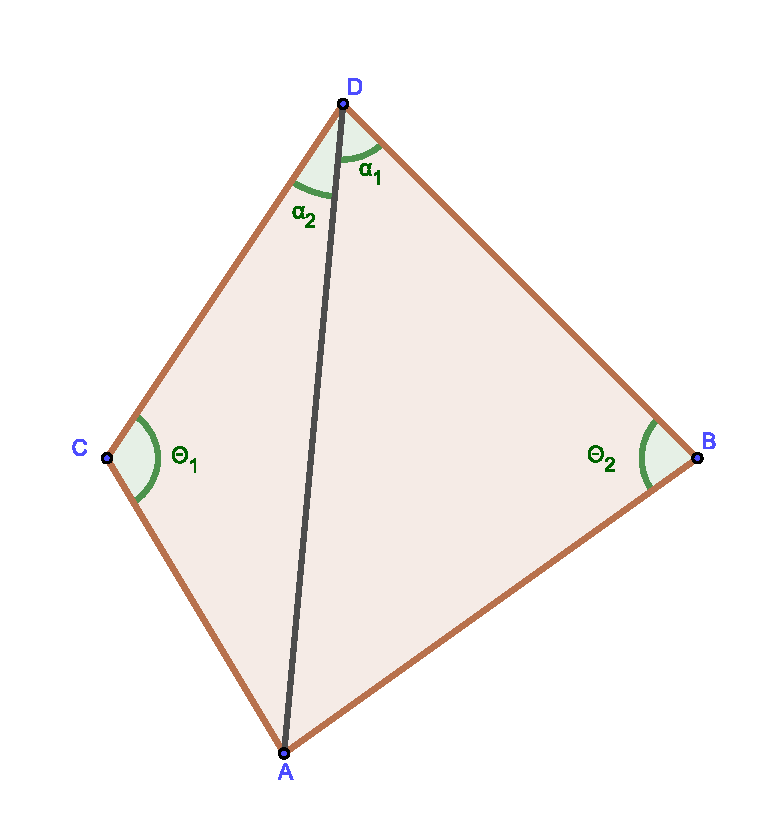
\includegraphics[width=0.35\linewidth]{pic/case3+.eps}
  \caption{区域III典型图}
  \label{区域III典型图}
  \end{figure} 


无论D点在$\Delta ABC$内部还是外部,所建立的方程保持不变。

\begin{equation}
    \left\{
              \begin{array}{ll}
                \theta_1+\theta_2=2\pi-(\alpha_1+\alpha_2+\alpha_3)\\
                \frac{sin\theta_1}{l}=\frac{sin\alpha_1}{r}=k_1\\
                \frac{sin\theta_2}{l}=\frac{sin\alpha_2}{r}=k_2\\

              \end{array}
            \right.
\end{equation}
\[
    \Rightarrow \theta_1=arctan \frac{-sin(\alpha_1+\alpha_2+\alpha_3)}{\frac{sin\alpha_2}{sin\alpha_1}+cos(\alpha_1+\alpha_2+\alpha_3)}
\]
或$\theta_1=90^{\circ}$。

若B的极坐标为(100,$\beta$),则该种情况下,未知点的定位坐标为(100$\times\frac{sin\theta_1}{sin\alpha_1}$,$\beta +$($\pi$-$\theta_1$-$\alpha_1$))。


(2)若$\alpha_1$、$\alpha_2$之间存在包含关系,即D点落在II、IV区域,两种可能性如图\ref{区域II典型图}\ref{区域IV典型图}所示;

\begin{figure}[H]
  \begin{minipage}[t]{0.45\linewidth}
  \centering
  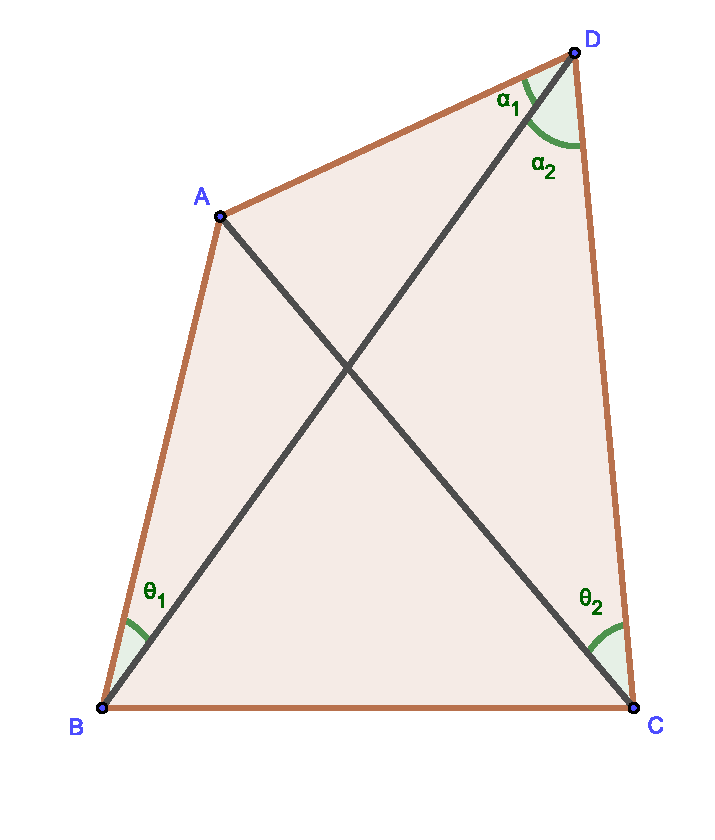
\includegraphics[height=5.5cm,width=5.5cm]{pic/case4.eps}
  \caption{区域II典型图}
  \label{区域II典型图}
  \end{minipage}%
  \begin{minipage}[t]{0.45\linewidth}
  \centering
  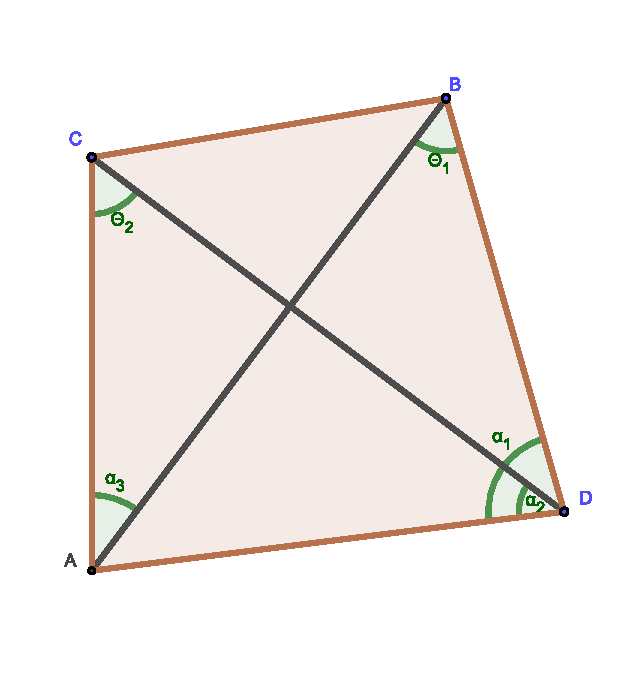
\includegraphics[height=5.5cm,width=5.5cm]{pic/case2+.eps}
  \caption{区域IV典型图}
  \label{区域IV典型图}
  \end{minipage}
  \end{figure}


当$\alpha_1 < \alpha_2$时:

\begin{equation}
    \left\{
              \begin{array}{ll}
                \theta_1-\theta_2=\alpha_2-(\alpha_1+\alpha_3)=\theta_0\\
                \frac{sin\theta_1}{l}=\frac{sin\alpha_1}{r}=k_1\\
                \frac{sin\theta_2}{l}=\frac{sin\alpha_2}{r}=k_2\\

              \end{array}
            \right.
\end{equation}

\[
    \Rightarrow \theta_1=arctan\frac{sin\theta_0}{cos\theta_0-\frac{sin\alpha_2}{sin\alpha_1}},\theta_0=\alpha_2-(\alpha_1+\alpha_3)
\]
或$\theta_1=90^{\circ}$。

若B的极坐标为(100,$\beta$),则该种情况下,未知点的定位坐标为(100$\times\frac{sin\theta_1}{sin\alpha_1}$,$\beta +$($\pi$-$\theta_1$-$\alpha_1$))。


当$\alpha_1 > \alpha_2$时:

\begin{equation}
    \left\{
              \begin{array}{ll}
                \theta_2-\theta_1=\alpha_1-(\alpha_2+\alpha_3)=\theta_0\\
                \frac{sin\theta_1}{l}={sin\alpha_1}{r}=k_1\\
                \frac{sin\theta_2}{l}={sin\alpha_2}{r}=k_2\\

              \end{array}
            \right.
\end{equation}

\[
    \Rightarrow \theta_1=arctan\frac{sin\theta_0}{\frac{sin\alpha_2}{sin\alpha_1}-cos\theta_0},\theta_0=\alpha_1-(\alpha_2+\alpha_3)
\]
或$\theta_1=90^{\circ}$。

若B的极坐标为(100,$\beta$),则该种情况下,未知点的定位坐标为(100$\times\frac{sin\theta_1}{sin\alpha_1}$,$\beta -$($\pi$-$\theta_1$-$\alpha_1$))。

由于$\theta_1$有四种不同的表达方式,故未知点仍有四个可能的坐标位置。 

\subsubsubsection{最终位置的确定}

由于我们无从知道D点究竟落在哪个区域,故四个点的坐标均有可能。然而题目中提及被动接收信号无人机所在位置仅略有偏差,故我们考虑将求解出来的四个坐标分别与标准坐标求欧几里得距离,将其中距离最短的点作为该无人机所在的位置。

距离公式计算方式如下:

设D点的标准坐标为(100,$\gamma_0$),求解出来的其中一个坐标为(100$\times\frac{sin\theta_1}{sin\alpha_1}$,$\beta \pm$($\pi$-$\theta_1$-$\alpha_1$)),则:

\[
 s=\sqrt{100^2+(100\times\frac{sin\theta_1}{sin\alpha_1})^2-2\times100\times(100\times\frac{sin\theta_1}{sin\alpha_1})\times cos(\gamma_0-\beta \pm(\pi-\theta_1-\alpha_1))}
\]

\subsubsection{几何模型的相关检验}

为了验证该位置确定方式的严谨性,我们进行了相关数据的模拟。随机选取两个编号的无人机作为发射源无人机,另外七个编号的无人机作随机扰动,使其略微偏离标准位置。由于我们采用的为极坐标系,所以给出一个扇形区域的误差限,但为了跟实际情况更加匹配,通过调整极径和幅角,使扇形区域尽可能接近方形区域。

经过相关计算,我们给出极径误差为$\pm 5m $,幅角误差为$\pm 3^{\circ}$,从而使得随机误差在10\%以内,且浮动区域约为一个方形,如图\ref{误差范围示意图}所示。

\begin{figure}[H]
  \centering
  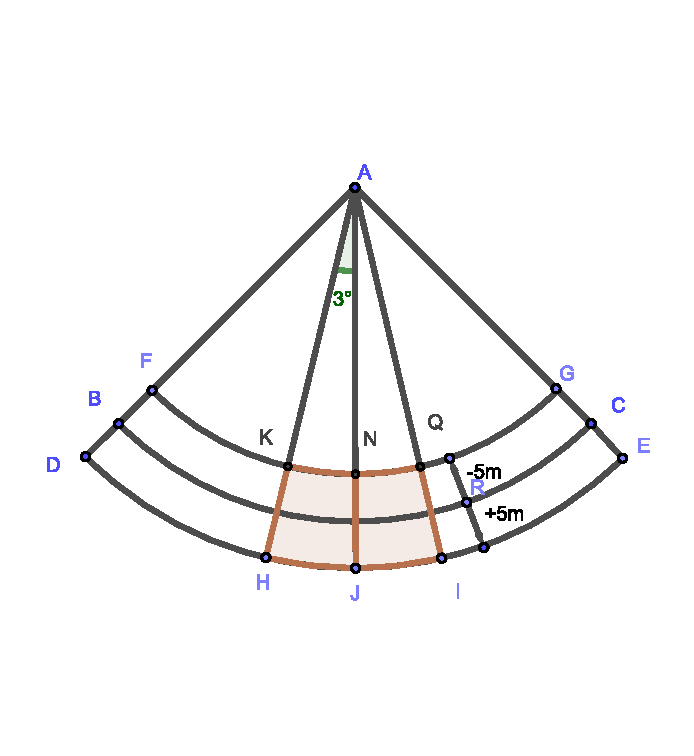
\includegraphics[width=0.45\linewidth]{pic/error area.eps}
  \caption{误差范围示意图}
  \label{误差范围示意图}
  \end{figure}

模拟方式为在9个编号点中选取其中3个,两个点为发射点,一个点为接收点,给接收点设置一个随机扰动,得到一组模拟真实数据。计算接收点与发射源间的方向信息后,将其作为输入,用上文所建的模型进行求解后,得到一组求解数据。用模拟真实数据与求解数据进行比较,以此判断模型的准确性。

选取方案总共有$\begin{pmatrix} 3 \\ 9 \end{pmatrix}\times 3=252$种,将其全模拟并且在随机扰动十万次后,发现模拟真实数据与求解数据间的误差在小数点10位之后,考虑为机器误差。由于数据量过大,故不将具体数据放入正文及附录中,具体内容可见于支撑材料。

\subsubsection{发射源的选取}

共有四类发射源的选取方式,分别与原点的夹角为$\pm 40^{\circ}$,$\pm 80^{\circ}$,$\pm 120^{\circ}$,$\pm 160^{\circ}$。

不断扩大误差范围,直至扩大到误差为30\%(即极径误差限扩大为$\pm 15m$,幅角误差限扩大为$\pm 3^{\circ}$时,出现“报错现象”。“报错现象”的定义为模拟真实位置与求解位置之间的距离超过机器误差eps(根据经验,约为$10^{-8}$)。

在上部分的模拟中,这四类情况我们均有涉及,现为扩大数据量,增加实验可信度,每轮模拟次数调整为10000000次。其中,发射源的圆心角为$40^{\circ}$时,报错概率较小,约为其他几类情况报错概率的$\frac{1}{2}$。

运行三轮的数据基本保持稳定,具体结果如下图\ref{不同发射源圆心角的报错频次图}所示:

\begin{figure}[H]
  \centering
  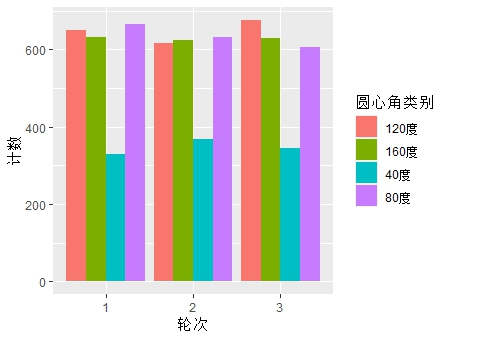
\includegraphics[width=0.55\linewidth]{pic/Rplot01.jpeg}
  \caption{不同发射源圆心角的报错频次图}
  \label{不同发射源圆心角的报错频次图}
  \end{figure}



故在进行发射源的选取时,可以尽可能多考虑圆心角为$40^{\circ}$的两个无人机作为发射源。


\subsection{问题二模型的建立与求解}

在信号源编号未知的情况下,每次多引入一个信号源,只能额外得到以接受信号无人机为顶点的两个有效角度信息。从几何求解角度,其不足以得到定位所需的极径、幅角。于是我们考虑利用已知角度信息先确定至少一架发射信号无人机的编号,即可把该问题等同于问题一,利用相同方法定位。

\subsubsection{角度区间定位模型}

\subsubsubsection{角度范围划定}
考虑以待定位无人机理想位置为顶点、FY01与另一未知编号无人机所发射信号为两边形成的圆周角,圆周上相邻的发射信号无人机对应的该角度有$20^{\circ}$的变化量。鉴于待定位无人机位置只是略有偏差,故不同发射信号无人机对应的该角度也只是相对理想圆周角略有改变,不同的信号源无人机形成的圆周角仍可认为处于不同的跨度为$20^{\circ}$的角度区间中。

对待定位无人机,根据每$20^{\circ}$对应一个信号来源无人机,对接受到的信号的角度进行线性区间划分。再根据实际测得的角度信息落入的角度区间,找到其对应的发射信号无人机,即可推定信号源无人机的编号。

又由于等长的弦对应的圆周角相等,故由上会得到两个关于过FY01的径向对称分布的均满足该角度情况的信号源无人机编号。

例如在FY04作为待定位无人机、FY03作为一发射信号无人机的情况下,接受到的信号近似圆周角为$38^{\circ}$,此时对各个不同信号源无人机位置,有对应角度划分区间如下表;

\begin{center}
  表2:各编号无人机作信号源时对应角度区间
  ~\\
    \begin{tabular}{|c|c|c|c|c|c|}
        \hline
        无人机编号&角度区间($^{\circ}$)&无人机编号&角度区间($^{\circ}$)&无人机编号&角度区间($^{\circ}$)\\
        \hline
        FY02&[0,30)&FY03&[30,50)&FY05&[70,90]\\
        \hline
        FY06&[70,90]&FY07&[50,70)&FY08&[30,50)\\
        \hline
        FY09&[0,30)& & & &\\    
        \hline
    \end{tabular}\\
\end{center}

该表由FY01作为起始零度点,向两侧每隔$20^{\circ}$进行划分得到。其中因为FY01作为已知的固定发射源存在,故将较小的角度区间直接划分给两侧的FY01、FY09。同时我们将可能的测得角为钝角情况考虑为一对优弧、劣弧对应的一对对称无人机情况,故表中直接考虑其补角即可。

在该情境下,测得的$38^{\circ}$落在了$[30,50)$划分区间,故由表可知其最可能的信号发射来源为FY03、FY08这一对无人机。

\begin{figure}[H]
  \centering
  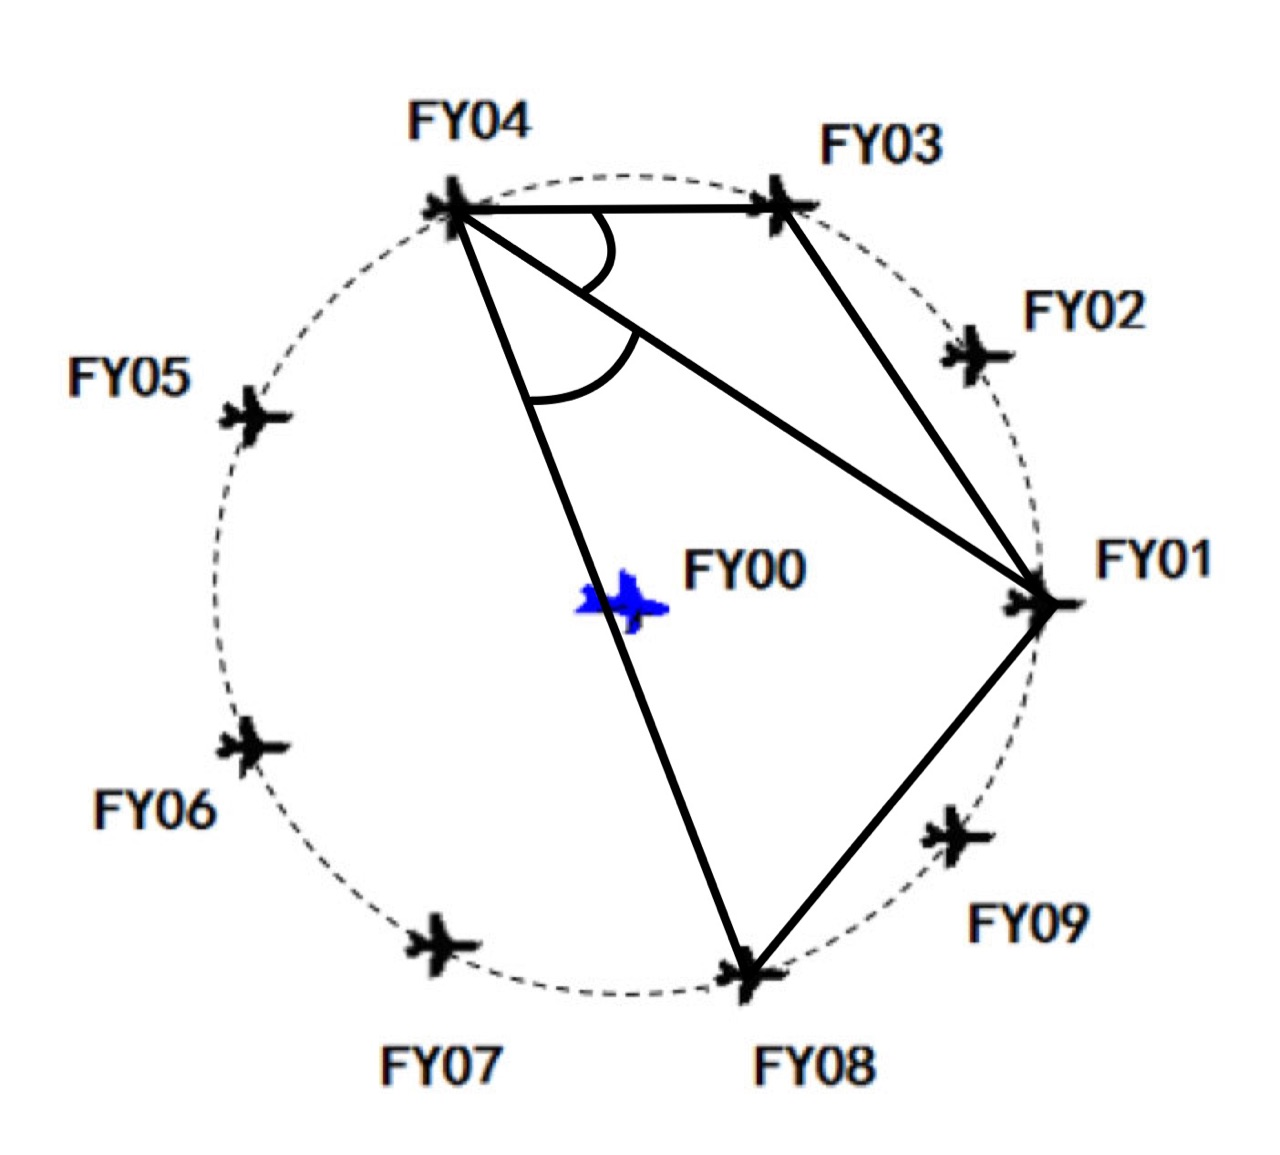
\includegraphics[height=5.5cm,width=5.5cm]{pic/example_for_2.a.jpg}
  \caption{接收信号角度示意图}
  \end{figure}



\subsubsubsection{对称点的判断}

当将获得的方向信息对应在相应的角度区间上时,我们可以判断未知发射源无人机的可能编号。编号的可能性一般有两种且关于FY01号无人机的位置对称,为了判别发射源无人机的真实编号,我们对其进行机理分析。

设需要判别的两个编号为$c_1$,$c_2$,其中$c_1+c_2=11$,在圆周上均匀分布着9个点,1个点为已知发射源FY01,2个点为可能发射源。这三个点上无人机的位置不存在偏差,根据对称特性,2个可能发射源与FY01中相隔点的数量相同,将这些相隔点定义为区内点。除去这三类点后,圆周上一定还存在偶数个点,并将这些点定义为区外点,具体定义如下图\ref{点的定义图}。接收信号的无人机的真实位置与这些点略有偏差。

\begin{figure}[H]
  \centering
  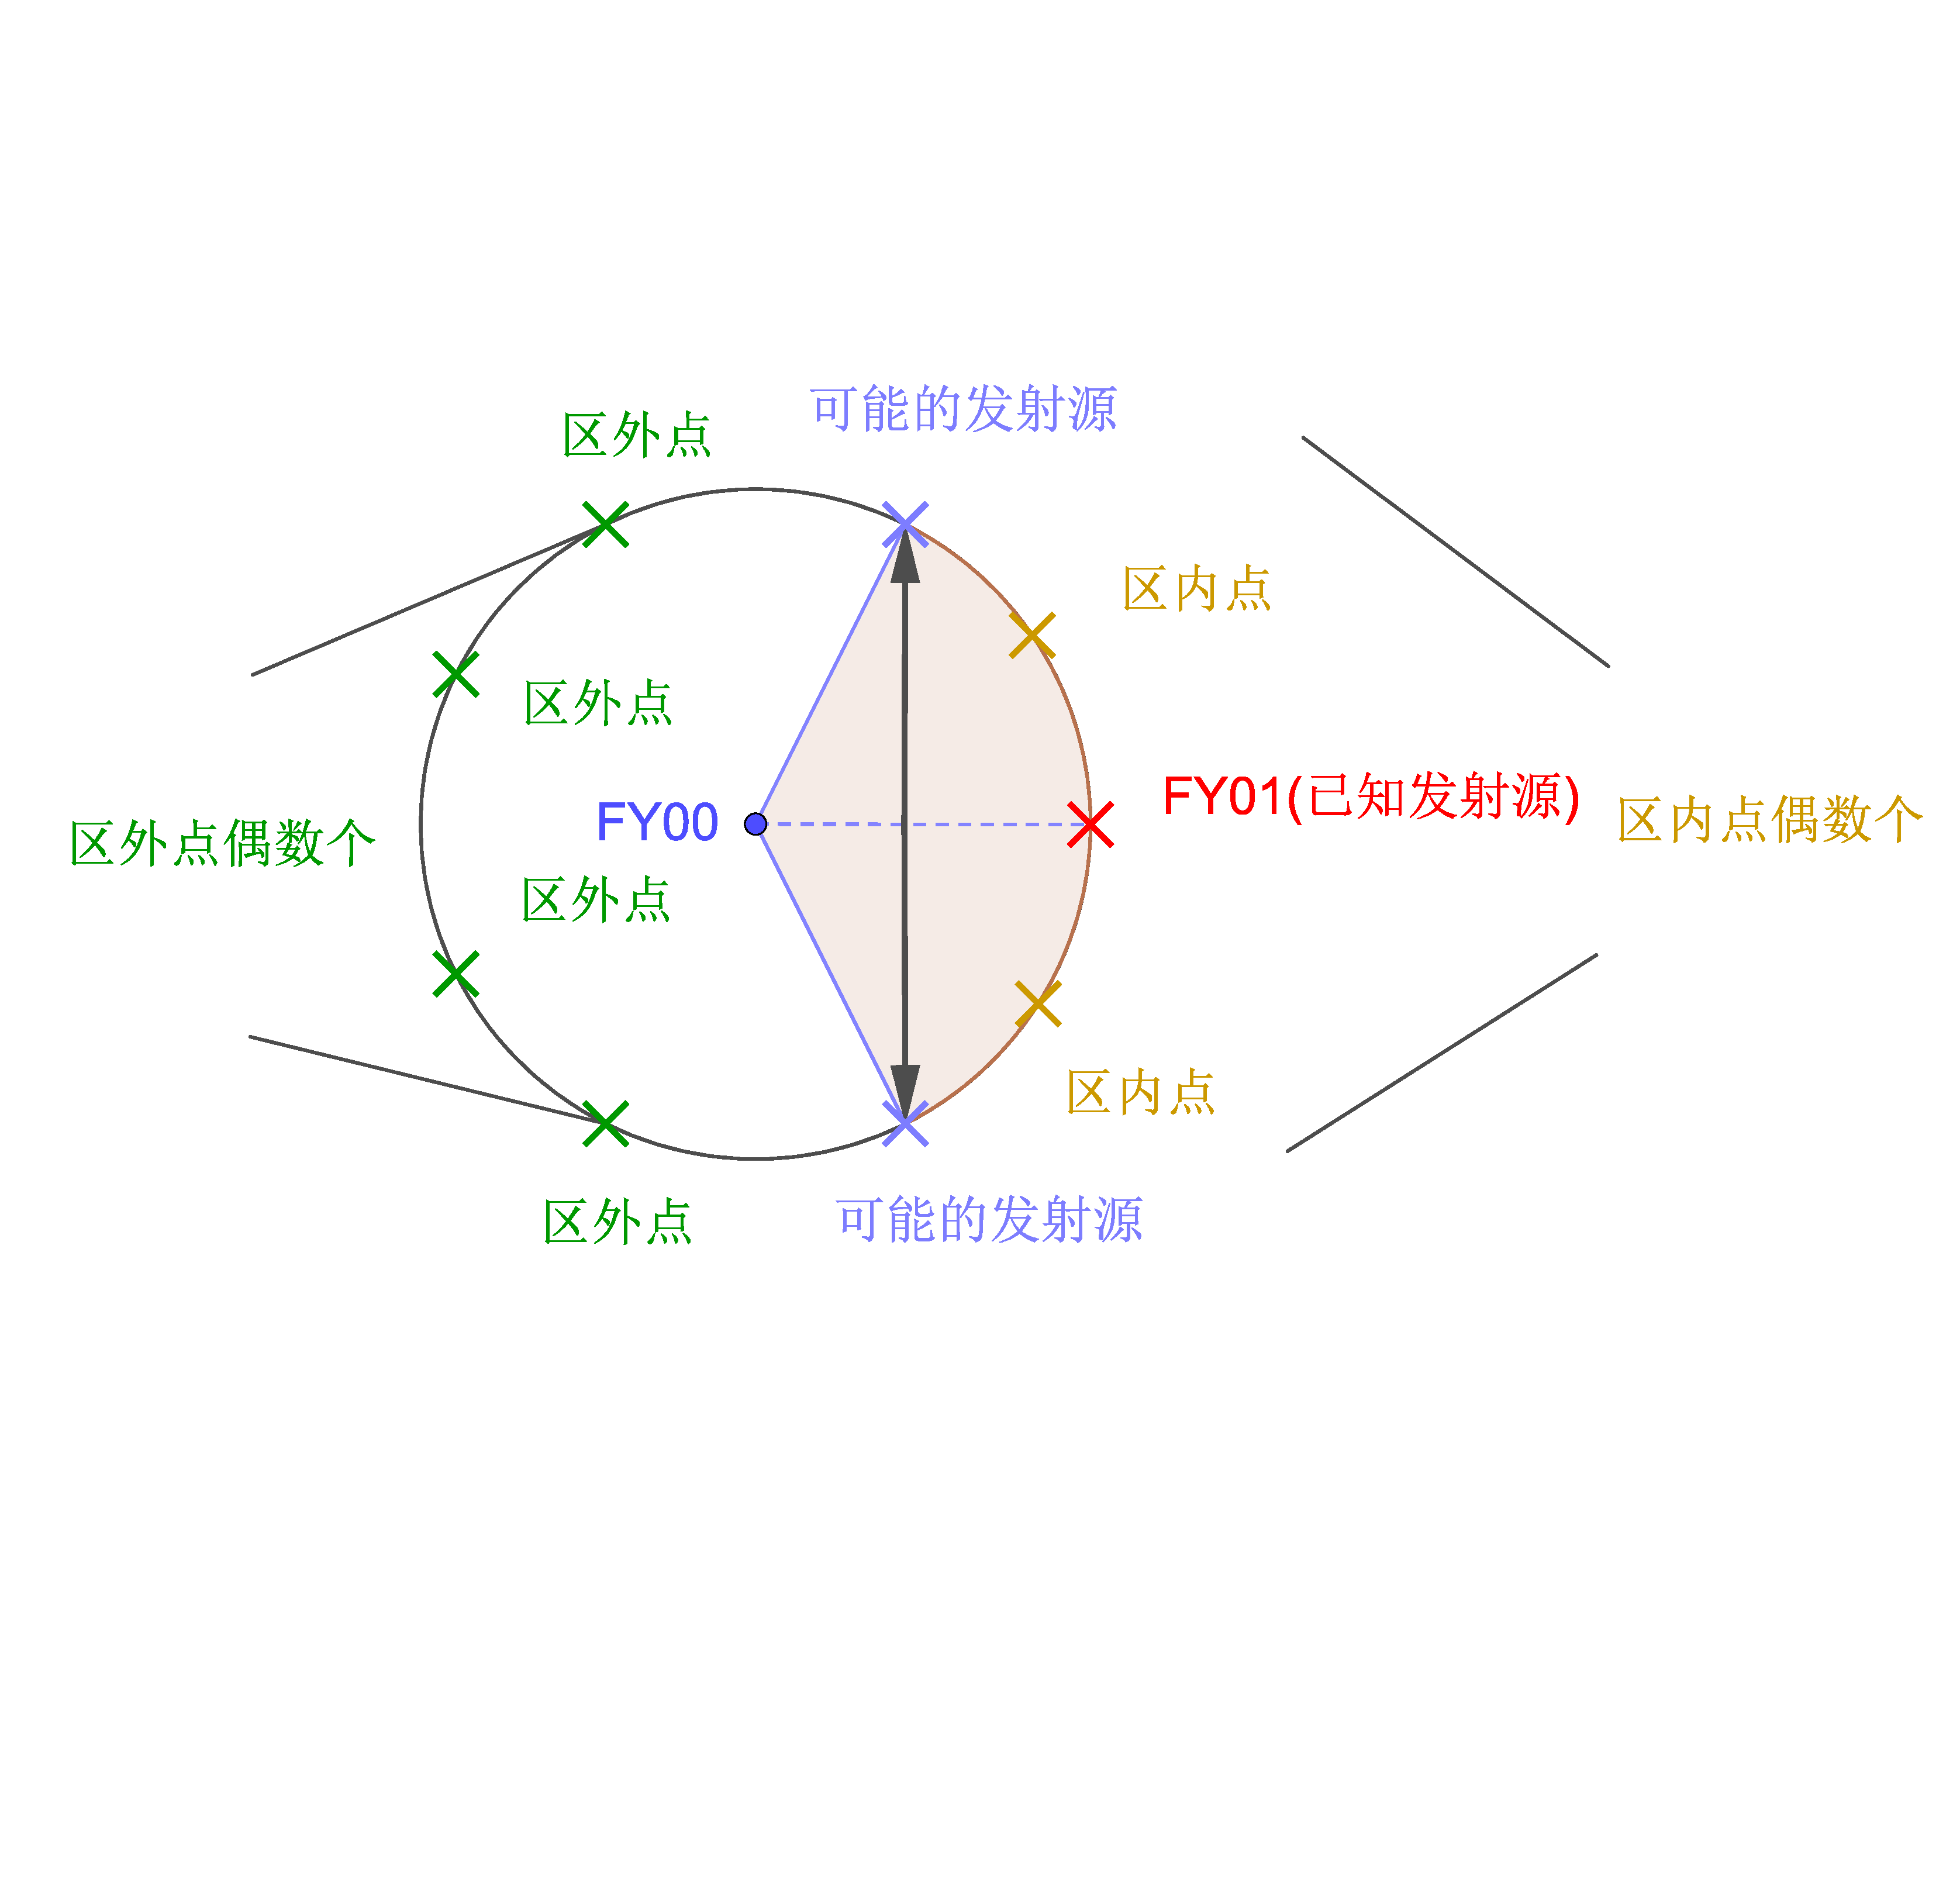
\includegraphics[width=0.55\linewidth]{pic/regional_points.eps}
  \caption{点的定义图}
  \label{点的定义图}
  \end{figure}


接收点存在的位置有两种可能,一种为区内点附近,一种为区外点附近。

为了更清晰地进行阐释,下面给出了两个典型情况的举例(左图为接收点在区内点附近,右图为接收点在区外点附近)。设接收点为FY02/FY06附近略有偏差的点,可能发射源为FY03和FY08。令FY00所在点为O,FY01为P,可能发射源分别为$F_1$、$F_2$,接收点为J,如下图\ref{区内点情况}\ref{区外点情况}所示。

\begin{figure}[H]
  \begin{minipage}[t]{0.45\linewidth}
  \centering
  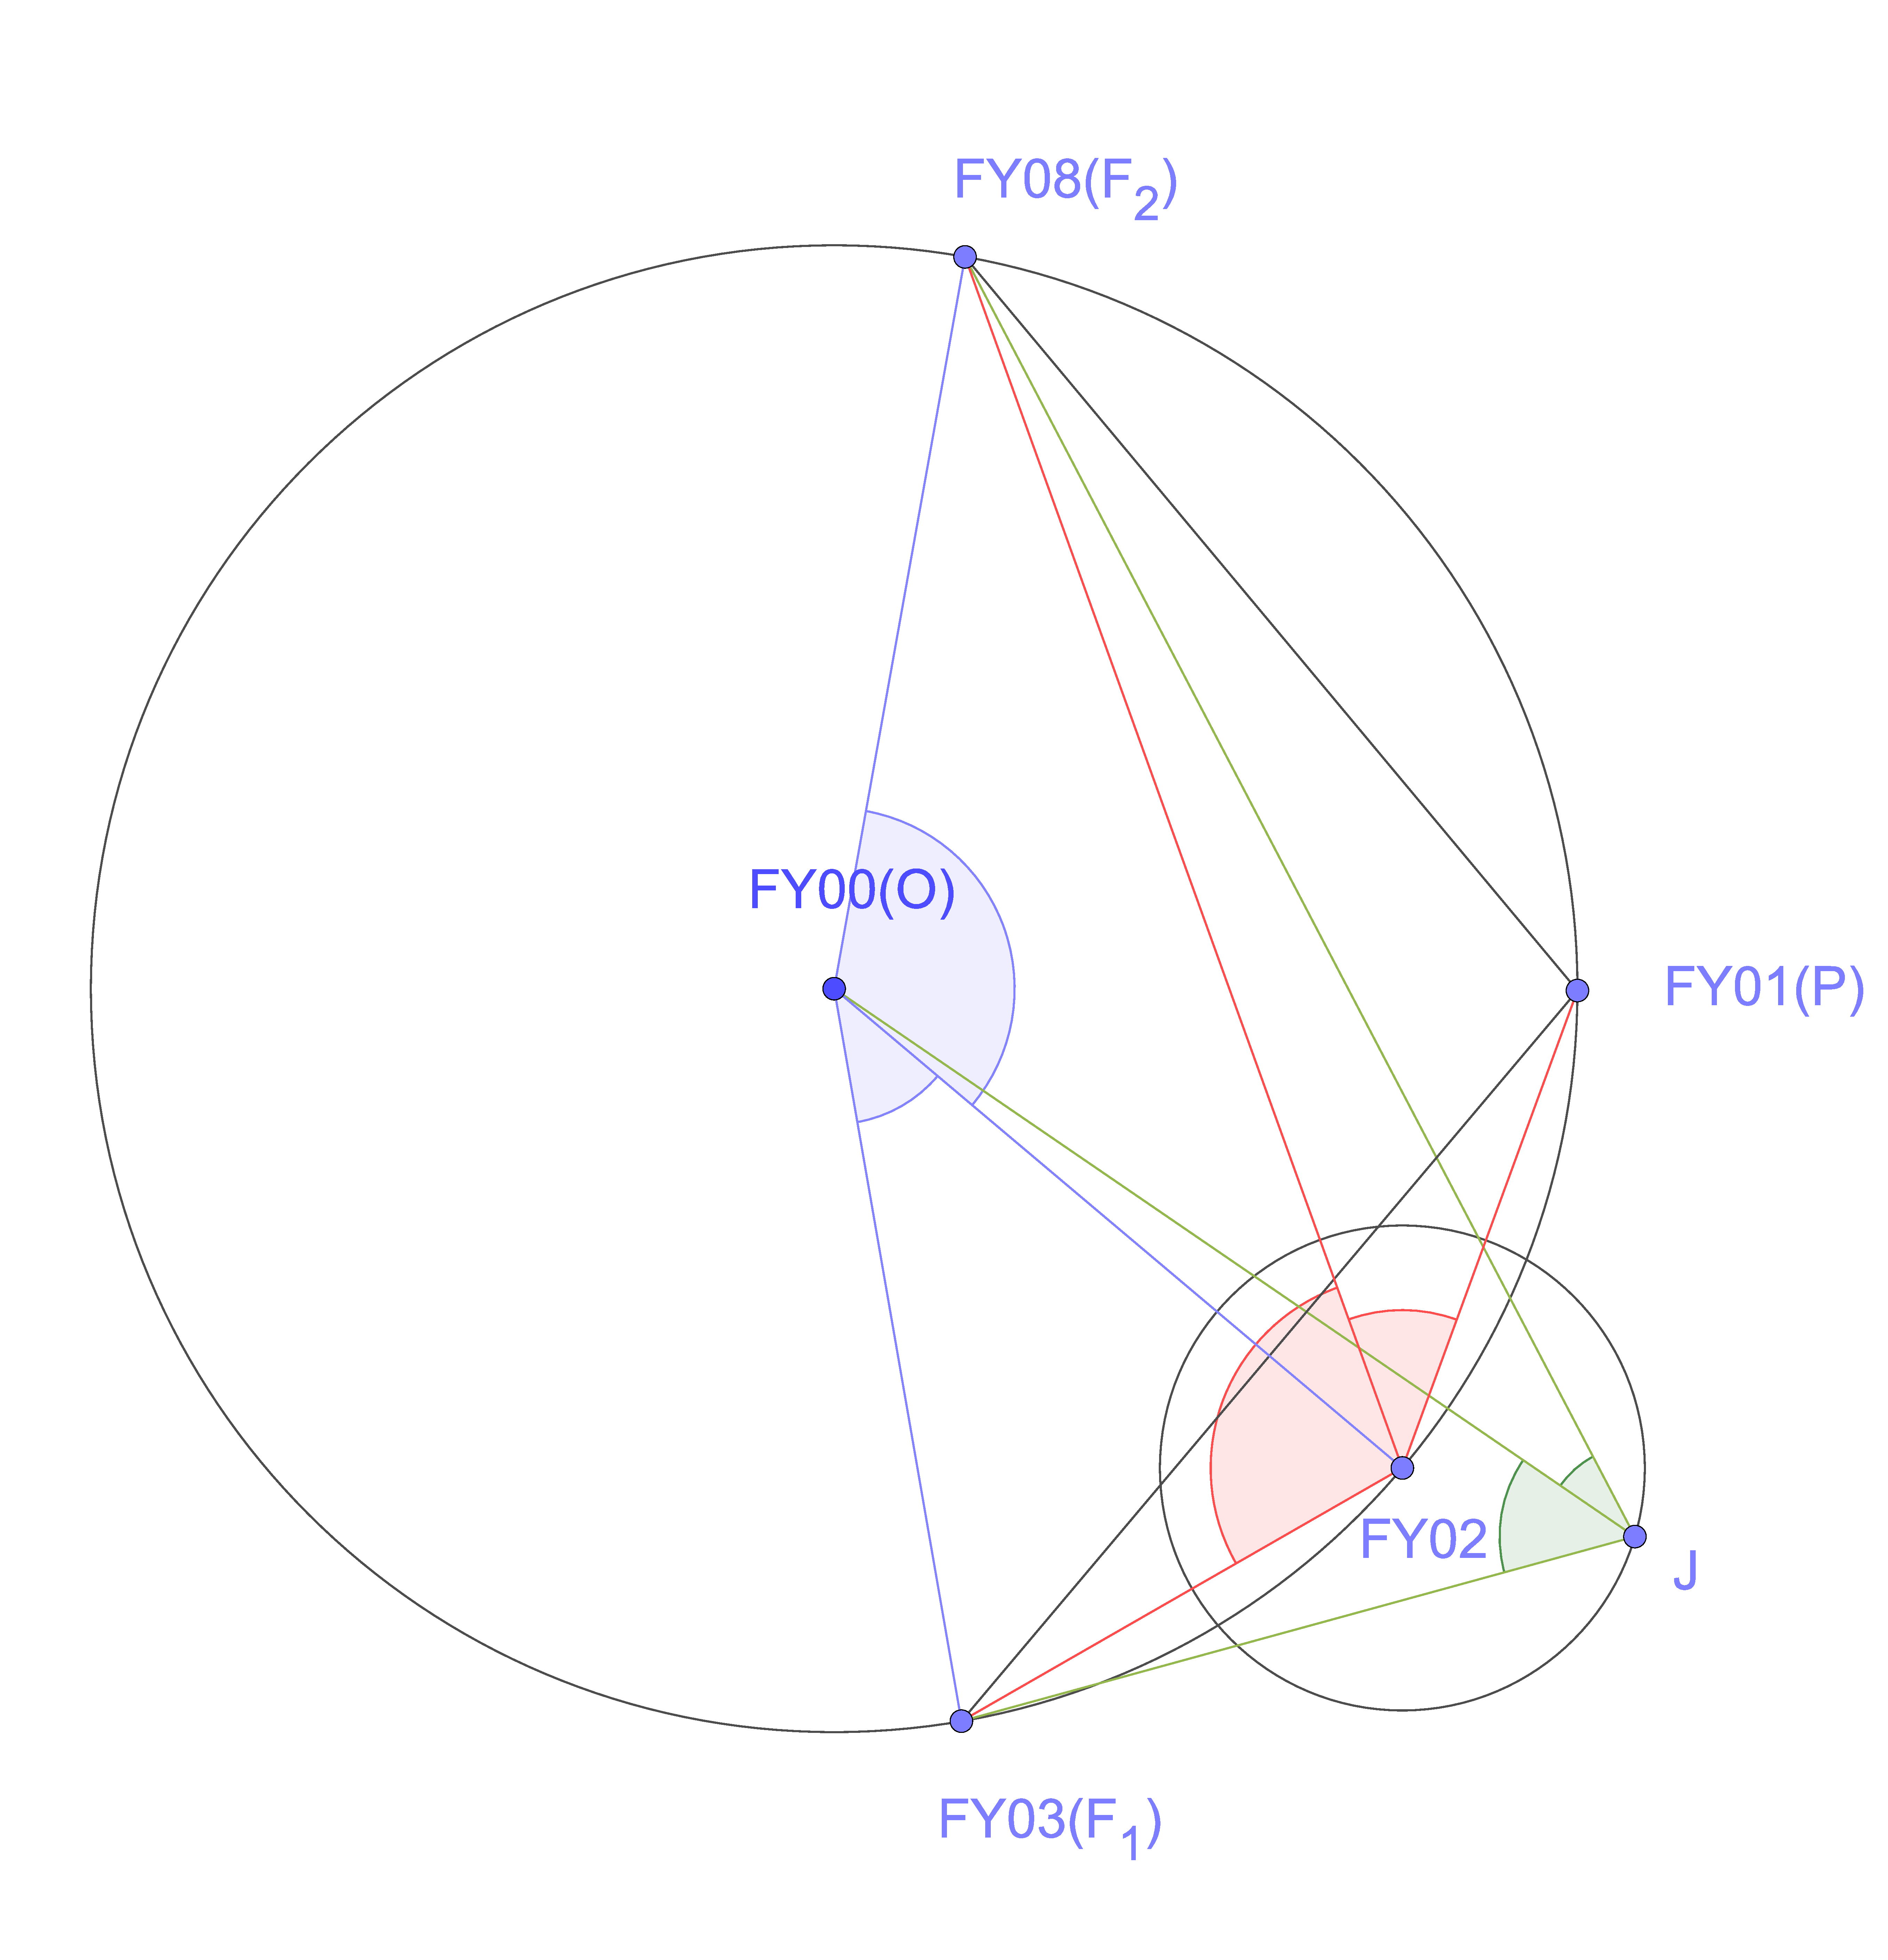
\includegraphics[height=5.5cm,width=5.5cm]{pic/error_circle1(1).eps}
  \caption{区内点情况}
  \label{区内点情况}
  \end{minipage}%
  \begin{minipage}[t]{0.45\linewidth}
  \centering
  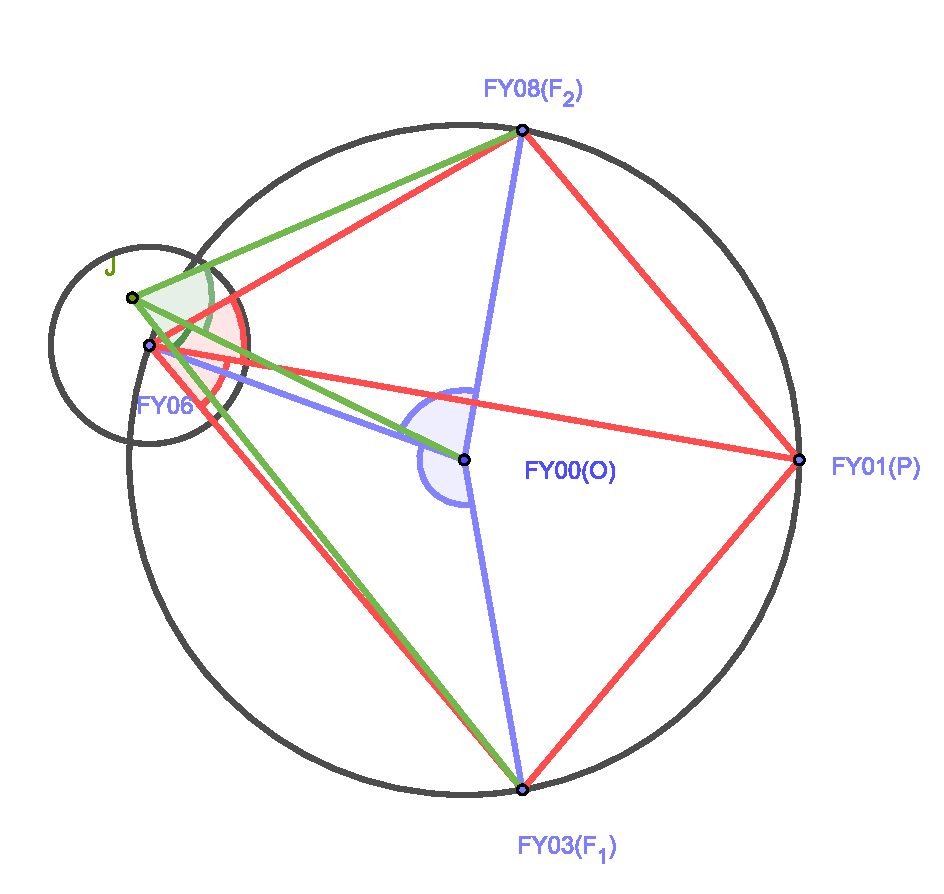
\includegraphics[height=5.5cm,width=5.5cm]{pic/error_circle2.eps}
  \caption{区外点情况}
  \label{区外点情况}
  \end{minipage}
  \end{figure}


由左图可以看出,P点等分了发射源包含的区间,由于接收点的位置仅略有偏差,我们不妨假设它就在J点上。显然,接收点仅能落在等分区间的其中一个上,区间内与两个可能发射源圆心角相同的点仅有P点,因此接收点与不同发射源之间的圆心角一定不同。

由右图可以看出,$F_1$,$F_2$之间不包含P点的弧被区外点划分成了奇数段(包括$F_1$,$F_2$共有偶数个点,首尾不相连,组成奇数个区间),J点将这奇数个区间再次进行划分,分为奇数段的区间及偶数段的区间。显然这两段区间对应的圆心角明显不同。

故我们采用FY00和可能发射源无人机给出的方向信息对编号进行鉴别(即$\angle OJF_1$或$\angle OJF_2$),由于$\Delta OJF_1$及$\Delta OJF_2$均近似为等腰三角形,故在圆心角不同的前提下,方向信息也不相同。比较真实得到的方向信息与两个理论角度,将与真实值更近的理论角度判为真,选择其对应的发射源为真实编号数。

\subsubsection{结果展示与误差分析}

算法流程大致分为以下两步:

\textbf{Step 1:}根据前文所建模型得出未知发射源的编号

\textbf{Step 2:}利用第一问的算法确定接收信号无人机的所在位置

与第一问相同,控制接收端的偏移误差在10\%以内,构造一个近似为方形的扇形区域,即极径误差为$\pm 5m $,幅角误差为$\pm 3^{\circ}$。

模拟方式为在9个编号点中选取其中2个,一个点为发射点,一个点为接收点,给接收点设置一个随机扰动,得到一组模拟真实数据。计算接收点与发射源间的方向信息后,将其作为输入,用算法进行求解后,得到算法给出的发射源求解编号以及接收端求解位置。将其与模拟真实数据进行比较,以此判断模型的准确性。

选取方案总共有$\begin{pmatrix} 2 \\ 9 \end{pmatrix}\times 2=72$种,将其全模拟并且在随机扰动一百万次后,发现报错率(即编号选取出错概率)为0。

为了检验模型可承受的误差范围,我们以0.1\%的间隔不断扩大偏移范围,发现在误差超过12\%之后,开始有“报错现象”的出现。

“报错现象”出现的原因有两类:第一类为未知编号判断错误,第二类为定位错误(可能源于未知编号判断错误,也可能是第一问的算法定位错误),也就是说,第一类错误的发生必将导致第二类错误的发生。

两类错误的具体报错概率如下图\ref{两类错误报错概率折线图}所示:

\begin{figure}[H]
  \center
  
  \subfigure[两类错误整体趋势]{
  \begin{minipage}[c]{0.55\linewidth} %自行调整,太大的话会自动换行
  \centering
  \includegraphics[width=0.85\linewidth]{pic/大.jpeg}
  %width相加大于1时自动换行
  %自行调整width \vsapce \hspace
  \end{minipage}
  }\hspace{-20pt}%调整subfigure的间距
  \subfigure[误差为39\%-40\%两类错误的差异及差异分界点]{
  \begin{minipage}[c]{0.40\linewidth}
  \centering
  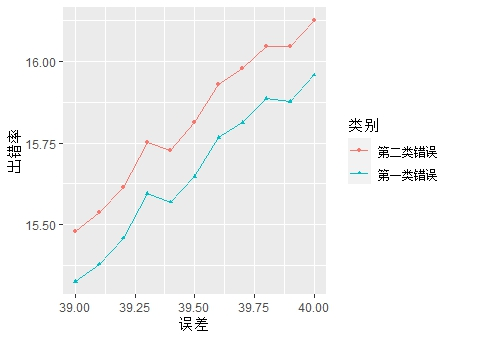
\includegraphics[width=1.00\linewidth]{pic/39.jpeg}\vspace{4pt}
  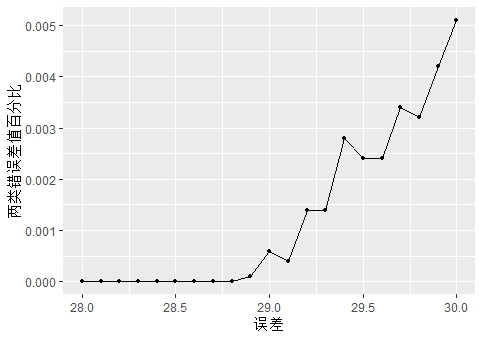
\includegraphics[width=0.75\linewidth]{pic/28.jpeg}
  \end{minipage}
  }
  \caption{两类错误报错概率折线图}
  \label{两类错误报错概率折线图}
  \end{figure}

  由图中所给信息可以看出,当误差大于12\%时,编号选取出现错误;而在误差为12\%-29\%时,定位错误完全由编号选取失误造成;当误差接近29\%时,由第一问算法求解造成的误差开始逐渐增大,但当误差范围达到40\%时,依然远远小于编号选取错误造成的定位误差。

  通过对比分析误差来源的类型-未知发射源编号确定错误/无人机位置定位错误后发现,该问所建的模型对“略微偏移”的要求更高。一旦需要定位的无人机偏移位移较大,定位模型有一定概率会失效。

  \subsubsubsection{误差来源}

  该模型编号选取错误主要来自两个方面:第一是角度划分区间确定可能发射源选取错误,第二是对称点选取错误。

  当接收端无人机离标准位置偏离较大时(超过$\pm 6m$ ),可能会不符合我们人为设定的角度划分区间及对称点的角度范围。

  为了使无人机定位有更高的精度,我们对模型进行进一步的修正。

  \subsubsection{投票机制模型的建立}

  前文模型建立过程中,一个较大的误差来源为角度划分区间过于死板,虽这样划分能在得到方向信息后直接确定未知发射源的编号(对称两点),较为简易。但当接收点偏移位移较大时,如图\ref{错误判断编号示例}所示。
  
  \begin{figure}[H]
    \centering
    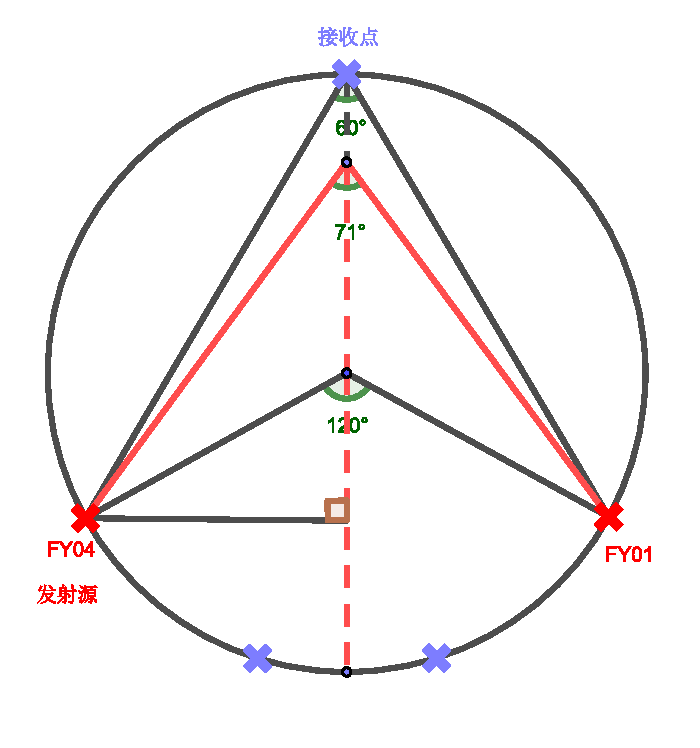
\includegraphics[width=0.35\linewidth]{pic/error.eps}
    \caption{错误判断编号示例}
    \label{错误判断编号示例}
    \end{figure}


  在这种情况下,本应是真正发射源的FY04,被误判成了FY05/FY06,导致错误。
  
  因此,我们决定在接收点的标准位置附近划定误差圆,通过误差圆来确定角度范围,但由于误差圆的半径选择依然较为主观,故我们选择用一系列大小不一的误差圆进行投票,以此确定未知发射源的编号。


  \subsubsubsection{角度范围的求解}

  由题意,无人机的真实位置在自身编号的标准位置附近,故我们以标准位置为中心作出误差圆。每一个可能的发射源(除无人机自身编号与FY01外,共有7个)均能根据误差圆得到一对判定的角度范围,具体求解如下:

  考虑待定位无人机J在一以理想位置Q为圆心、半径为r的误差圆内,其与FY01(P)、未知编号无人机(F)间形成的$\angle PJF$的,以及与FY01(O)形成的$\angle PJO$的大小为随J位置变化的函数。在确定二者关于J位置变化的区间后,即可对应找到唯一的同时满足两个角度区间的信号源无人机。

在求解两函数的变化区间时,可将问题考虑为一圆心在给定弦中垂线上变动,求变动的圆中该弦对应的圆周角的大小范围的等价命题。因为对给定弦,其所在的圆半径越大,对应的圆周角越小;因此当该动圆变动到恰与误差圆外切、内切时,半径取到最小、最大值,角度大小也相应取到最值。如在求解$\angle PJF$大小范围时,取最值的具体情形见下图:

  \begin{figure}[H]
    \begin{minipage}[t]{0.45\linewidth}
    \centering
    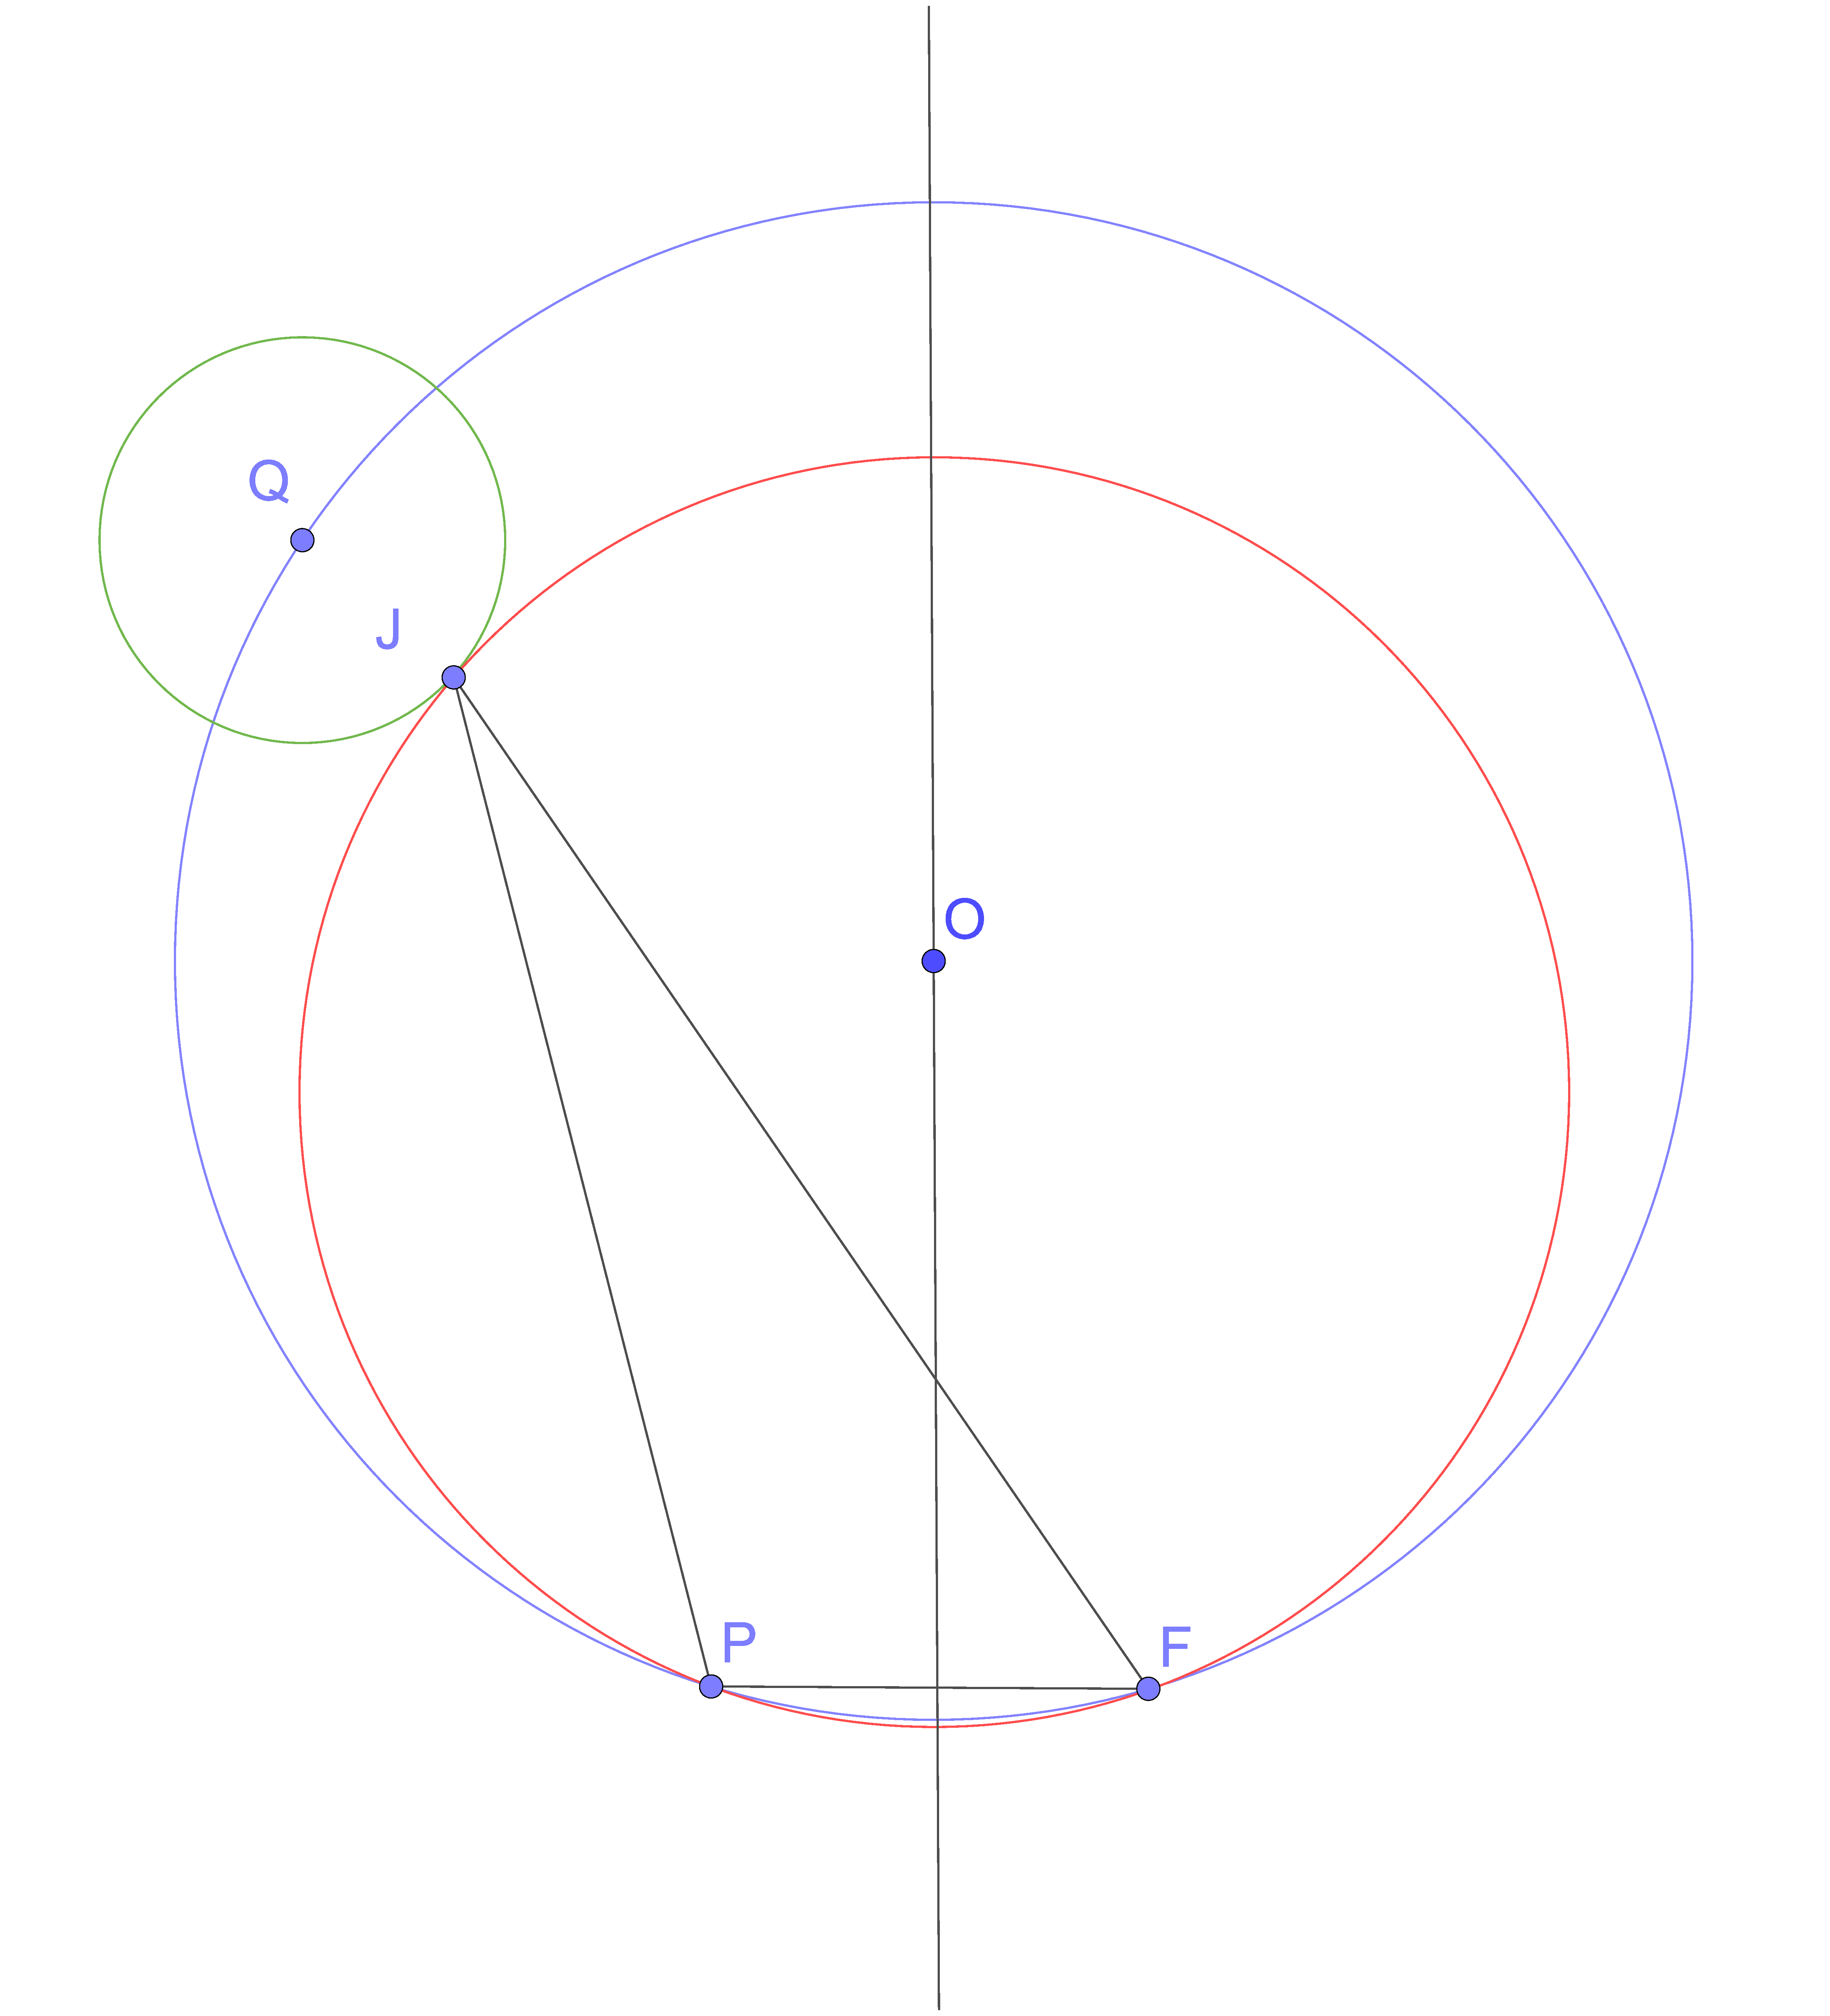
\includegraphics[height=5.5cm,width=5.5cm]{pic/angle_max.eps}
    \caption{$\angle PJF$最大值示意图}
    \end{minipage}%
    \begin{minipage}[t]{0.45\linewidth}
    \centering
    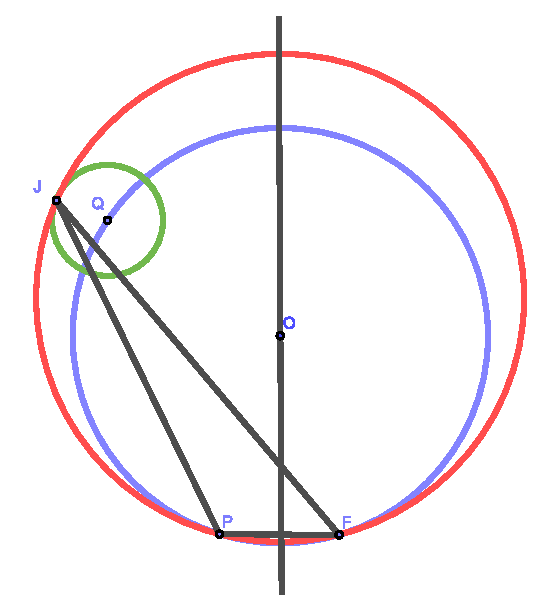
\includegraphics[height=5.5cm,width=5.5cm]{pic/angle_min.eps}
    \caption{$\angle PJF$最小值示意图}
    \end{minipage}
    \end{figure}


由于圆的凸性,两个角度大小的函数的最值一定在圆周上取到。因此虽然上述理论方法给出了准确求法,但在实际计算过程中,为了加快计算速度,我们采用了蒙特卡洛方法对其最值进行了可靠的估计。计算时先随机生成一个角度值,得到误差圆上对应角度的点的坐标,代入求解其对应的$\angle PJF$的大小。通过数次数值实验,我们采用1000次随机采样的最值来近似该函数的最值,经检验其具有良好的精确度。


  \subsubsubsection{误差圆的构造}

  由于接收端的真实位置是未知的,我们无法得出无人机具体被框定在哪个误差圆内,因此我们构造了半径为0.1m-40m,间隔为0.1m的400个同心圆,圆心均为接收信号无人机的标准位置。

  对每个误差圆均可求解得到可能发射源给出的一对角度范围,将其与接收端得到的方向信息进行比较,以此为基础进行投票。

  \subsubsubsection{投票机制}

  在正式投票前,我们可以得到一张已知信息表,其中包含误差圆Q的半径(范围为0.1m-40m);误差圆的圆心编号I(范围为2-9);可能发射源的编号F(范围为2-9);两个角度范围:包含FY00(O)点的角度范围$(O_{min},O_{max})$及包含FY01(P)点的角度范围$(P_{min},P_{max})$。

  由于数据条数过大,该表暂不放在正文中。

  我们让每个接收点标准位置$I$为圆心的误差圆根据接收点得到的角度信息进行投票,根据票数多少选择最可能的发射源$F_1$。

  设真实的发射源为$Ftrue_1$,则当接收点$J$得到了$\angle OJFtrue_1$和$\angle PJFtrue_1$的角度信息后,对于每个发射源$F$,它的得票数$vote_F$可由下列等式计算得到:

  \begin{equation}
  vote_F=\mathop{\Sigma}\limits_{Q} [V_{Q,I,F,Omin} \le \angle OJFtrue_1 \le V_{Q,I,F,Omax}][V_{Q,I,F,Pmin} \le \angle PJFtrue_1 \le V_{Q,I,F,Pmax}]
\end{equation}


  即400个误差圆中,每个误差圆都根据接收点得到的角度信息是否在每个发射源对应的角度区间内,可以给最少$0$个(角度信息不在任何发射点对应的角度区间内),最多$7$个(角度信息在除了已知发射源$P$和接收点标准位置$I$的所有发射源对应的角度区间内)发射源投票,最后我们将票数最高的发射源作为$F_1$,即:

  \begin{equation}
F_1=\mathop{\arg\min}\limits_{F} vote_F
\end{equation}




  \subsubsection{结果展示}

  为了检验模型的正确性,我们同样进行模拟检验。与上文中角度区间定位模型的模拟方式相同。即:在9个编号点中选取其中2个,一个点为发射点,一个点为接收点,给接收点设置一个随机扰动,得到一组模拟真实数据。计算接收点与发射源间的方向信息后,将其作为输入,用算法进行求解后,得到算法给出的发射源求解编号以及接收端求解位置。将其与模拟真实数据进行比较,以此判断模型的准确性。

  同样以0.1\%的间隔不断扩大偏移范围,发现在误差超过20.7\%(极径误差为$\pm 10m $,幅角误差为$\pm 6^{\circ}$)之后,才开始有“报错现象”的出现,相较前一个模型有明显提升。

  对上文中提到的两类错误重新作图\ref{两类错误报错概率折线图}分析如下:

  \begin{figure}[H]
  \center
  
  \subfigure[两类错误整体趋势]{
  \begin{minipage}[c]{0.60\linewidth} %自行调整,太大的话会自动换行
  \centering
  \includegraphics[width=1.00\linewidth]{pic/大1.png}
  %width相加大于1时自动换行
  %自行调整width \vsapce \hspace
  \end{minipage}
  }\hspace{-20pt}%调整subfigure的间距
  \subfigure[误差为39\%-40\%两类错误的差异及差异分界点]{
  \begin{minipage}[c]{0.40\linewidth}
  \centering
  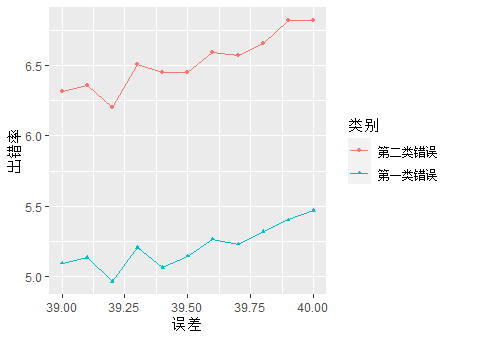
\includegraphics[width=1.00\linewidth]{pic/39.png}\vspace{4pt}
  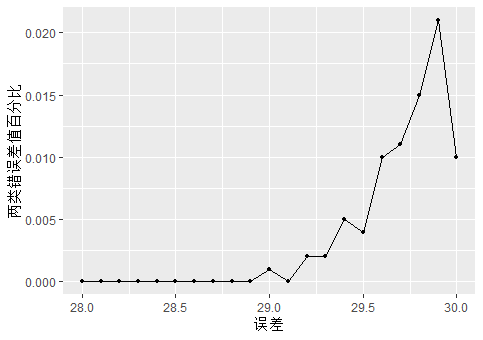
\includegraphics[width=0.75\linewidth]{pic/28.png}
  \end{minipage}
  }
  \caption{两类错误报错概率折线图}
  \label{两类错误报错概率折线图}
  \end{figure}

  由图中所给信息可以看出,当误差大于21\%时,编号选取出现错误;而在误差为21\%-29\%时,定位错误完全由编号选取失误造成;但整体而言,用投票机制构建的模型求解的效果远远好于角度区间定位模型。

  现在我们只增加了一架未知编号的发射源无人机提供方向信息,当误差达到40\%时,依然有近7\%的定位错误的可能。为了进一步提高精度,我们可以考虑多引入一架无人机。

  \subsubsubsection{进一步的思考}

  虽然投票机制令计算接收点位置错误的概率大大降低,但在接收点随机误差在40\%的范围内浮动时,仍有$6.821\%$的定位错误,而其中大部分($5.469\%$)是由于发射点编号确定出错导致的,故需要进一步优化模型,提高计算发射点编号的正确率。

  考虑加入第二架位置编号的发射信号的无人机$Ftrue_2$,接收点$J$还将得到$\angle OJFtrue_2$和$\angle PJFtrue_2$的角度信息,那么我们可以给所有可能的发射源对投票,以确定最可能的发射源对$F_1,F_2$。

  那么利用类似之前的投票方法,我们可以用以下等式计算每个点对的得票数:
\begin{equation}
\begin{split}
    vote_{F,F^{'}}=\mathop{\Sigma}\limits_{Q} [V_{Q,I,F,Omin} \le \angle OJFtrue_1 \le V_{Q,I,F,Omax}][V_{Q,I,F,Pmin} \le \angle PJFtrue_1 \le V_{Q,I,F,Pmax}]\\
    [V_{Q,I,F^{'},Omin} \le \angle OJFtrue_2 \le V_{Q,I,F^{'},Omax}][V_{Q,I,F^{'},Pmin} \le \angle PJFtrue_2 \le V_{Q,I,F^{'},Pmax}]
\end{split}
\end{equation}

即400个误差圆中,每个误差圆都根据接收点得到的角度信息是否在每个发射源对应的角度区间内,可以给最少$0$对,最多$7*6=42$对发射源投票,最后我们将票数最高的发射源作为$F_1,F_2$,即:
\begin{equation}
 F_1,F_2=\mathop{\arg\min}\limits_{F,F^{'}} vote_{F,F^{'}}
\end{equation}

为了减少通信资源浪费,我们将尽量使用一个未知编号发射源进行定位,当定位失败后,才考虑使用第二个未知编号发射源;但由于实际应用时无法得知真实坐标,故我们不能通过计算真实位置$J$和算法结果$J_0$之间的差值$|J-J_0|$来判断是否定位成功,故我们通过算法结果导出应得的角度信息$\angle OJ_0F_1$和$\angle PJ_0F_1$和真实数据比较来判断是否定位失败,即当$|\angle OJ_0F_1 - \angle OJFtrue_1| > eps$或$|\angle PJ_0F_1 - \angle PJFtrue_1| > eps$时判断为定位失败,再调用二轮投票模型来进行进一步的定位。

为了验证模型正确性,我们用和上文角度区间定位模型与投票机制模型的模拟方法相同的模拟方式进行模拟。将三种模型的报错情况作图\ref{三种模型报错概率折线图}如下:

\begin{figure}[H]
    \centering
    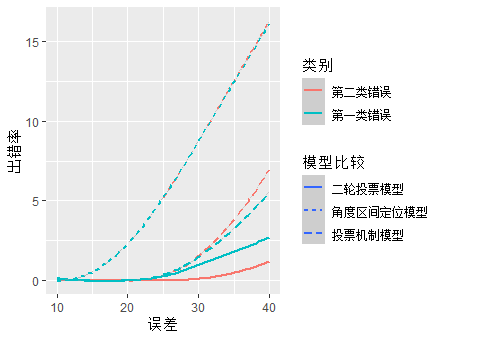
\includegraphics[width=0.60\linewidth]{pic/三类比较.png}
    \caption{三种模型报错概率折线图}
    \label{三种模型报错概率折线图}
\end{figure}

不难看出二轮投票模型的报错率明显低于其他两个模型,甚至能够在计算出的发射点不完全正确的情况下得出正确的定位信息(数据表现为第一类错误率大于第二类错误率),模型优化效果明显。

在模拟时,我们也记录了两种判断定位失败的方法判断的结果,发现在所有模拟中两种方法计算得出的定位失败率都相同,故可以证明用角度判断定位准确度的正确性。(具体结果可以查看支撑文件)



\subsection{问题三模型的建立与求解}
由于该问的整体流程和思路较为复杂,故绘制流程图\ref{问题三流程图}如下:

\begin{figure}[H]
  \centering
  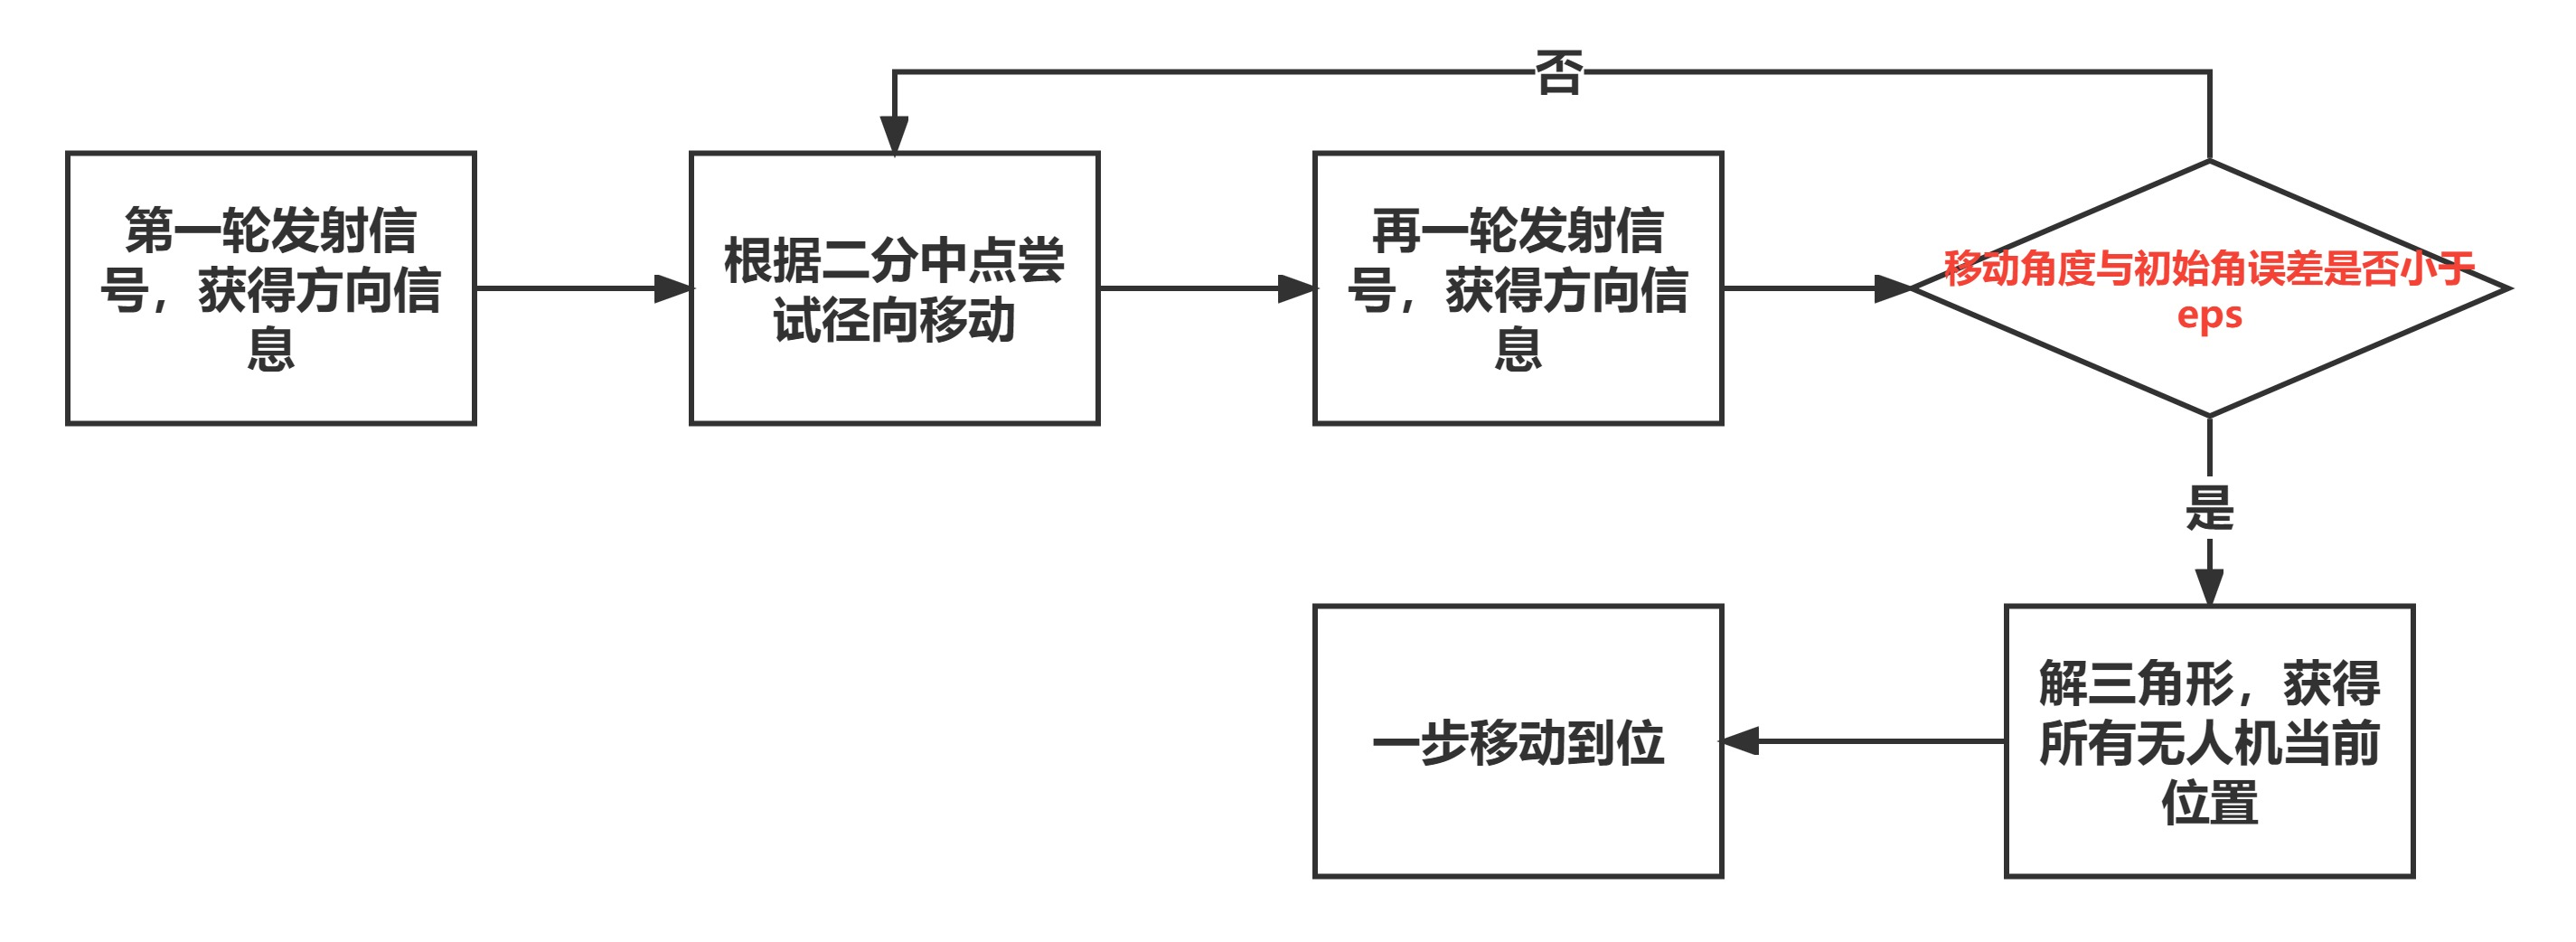
\includegraphics[width=0.85\linewidth]{pic/流程图(1).jpg}
  \caption{问题三流程图}
  \label{问题三流程图}
  \end{figure}
  \subsubsection{坐标系的建立}

由于现实场景中无人机水平方向的操纵命令往往是经由进退、左右式给出的,因此在本题中考虑建立坐标系描述无人机的运动过程时,选取了更贴近其运动形式的直角坐标系。

同时为了便于描述无人机的运动,我们进一步选取无人机的“前进”方向作为x轴的正方向,其“左转”方向作为y轴的正方向,并将原点定在位于机群中心的FY00处。同时为了便于后续整体队形的调整,我们将FY01的理想位置定于(100,0)。而由题目所给图片机群的机头朝向,我们假定机群前进方向即x轴方向。再根据题目给出的初始时刻无人机位置仅略有偏差,在此坐标系下FY01的实际位置与设定的理想位置(100,0)相距不远,故所建立的坐标体系合理。

  \subsubsection{信号发射机次的选取}
  为了方便每驾无人机的幅角方向的确定,我们考虑先通过无人机之间的信号传输得到每架无人机J与OP的夹角$\angle POJ$。具体地我们选取如下的信号发射机次方案:

  \begin{center}
  表3:各轮次选取的进行信号发射的无人机编号
  ~\\
    \begin{tabular}{|c|c|c|c|c|}
        \hline
        &轮次一&轮次二&轮次三&轮次四\\ 
        \hline
        发射信号无人机编号&(0,1)&(0,2,3,4)&(0,5,6,7)&(0,8,9)\\
        \hline
    \end{tabular}\\
  \end{center}

在第一轮次中,选取FY00、FY01作为发射信号的无人机,其余无人机均作为接受信号的无人机。由此可以得到所有以其余无人机位置为顶点、与(FY00,FY01)两点构成的$\angle OJP$的角度值。

后续三轮次中依旧保留了FY00,再选取了除FY00、FY01外其他的无人机依次来发射信号。其中重点考虑FY01接收到的角度信息,即以其为顶点的$\angle OPJ$。

结合各轮次信息,对除FY00、FY01外的无人机J,在$\Delta JOP$中即可求得圆心角。

\subsubsection{二分移动路径法}

首先我们需要确定圆周上的每架无人机到原点的连线和x轴的夹角大小,现在以编号为$FY02$的无人机为例说明如何确定该夹角大小。

  设$FY1,FY2$分别为$FY01$和$FY02$的理想位置,$FY1^{'},FY2^{'}$分别为$FY01$和$FY02$的真实位置,坐标原点为$O$,则$\alpha$为$OFY1^{'}$和$OFY2^{'}$两边的初始夹角。设$FY2^{''}$是$FY02$调整后的位置,则$\alpha^{'}$为$OFY1^{'}$和$OFY2^{''}$的夹角。
  若有$\alpha = \alpha^{'}$,说明$FY2^{''}$在$OFY2^{'}$的延长线上。令$FY2^{''}$在以$FY2^{'}$为圆心,常数$r$(具体实现时设置为$1m$)为半径的圆上调整。尽管我们初始时无法知道$FY2^{'}$的精确位置,但通过$r$和$\theta$容易计算$FY2^{'}$到$FY2^{‘'}$的变化量,故可以使用形式为$(\Delta x,\Delta y)$的调整指令使无人机在圆周上调整。
  
  设$FY2^{''}FY2^{'}$与x轴的夹角为$\theta$,则$\theta$和$\alpha^{'}$之间存在一个函数映射关系$\alpha^{'}=f(\theta)$,那么$FY2^{'}$的方向确定问题就转化为了$\alpha=f(\theta)$的方程求解问题。根据$FY02$的理想位置划定$\theta$的大致区间$[40^{\circ}-20^{\circ},40^{\circ}+20^{\circ}]$后,不难发现在此范围内$f(\theta)$是单调的,那么我们就可以使用二分法求解$\alpha=f(\theta)$。

  \begin{figure}[H]
    \centering
    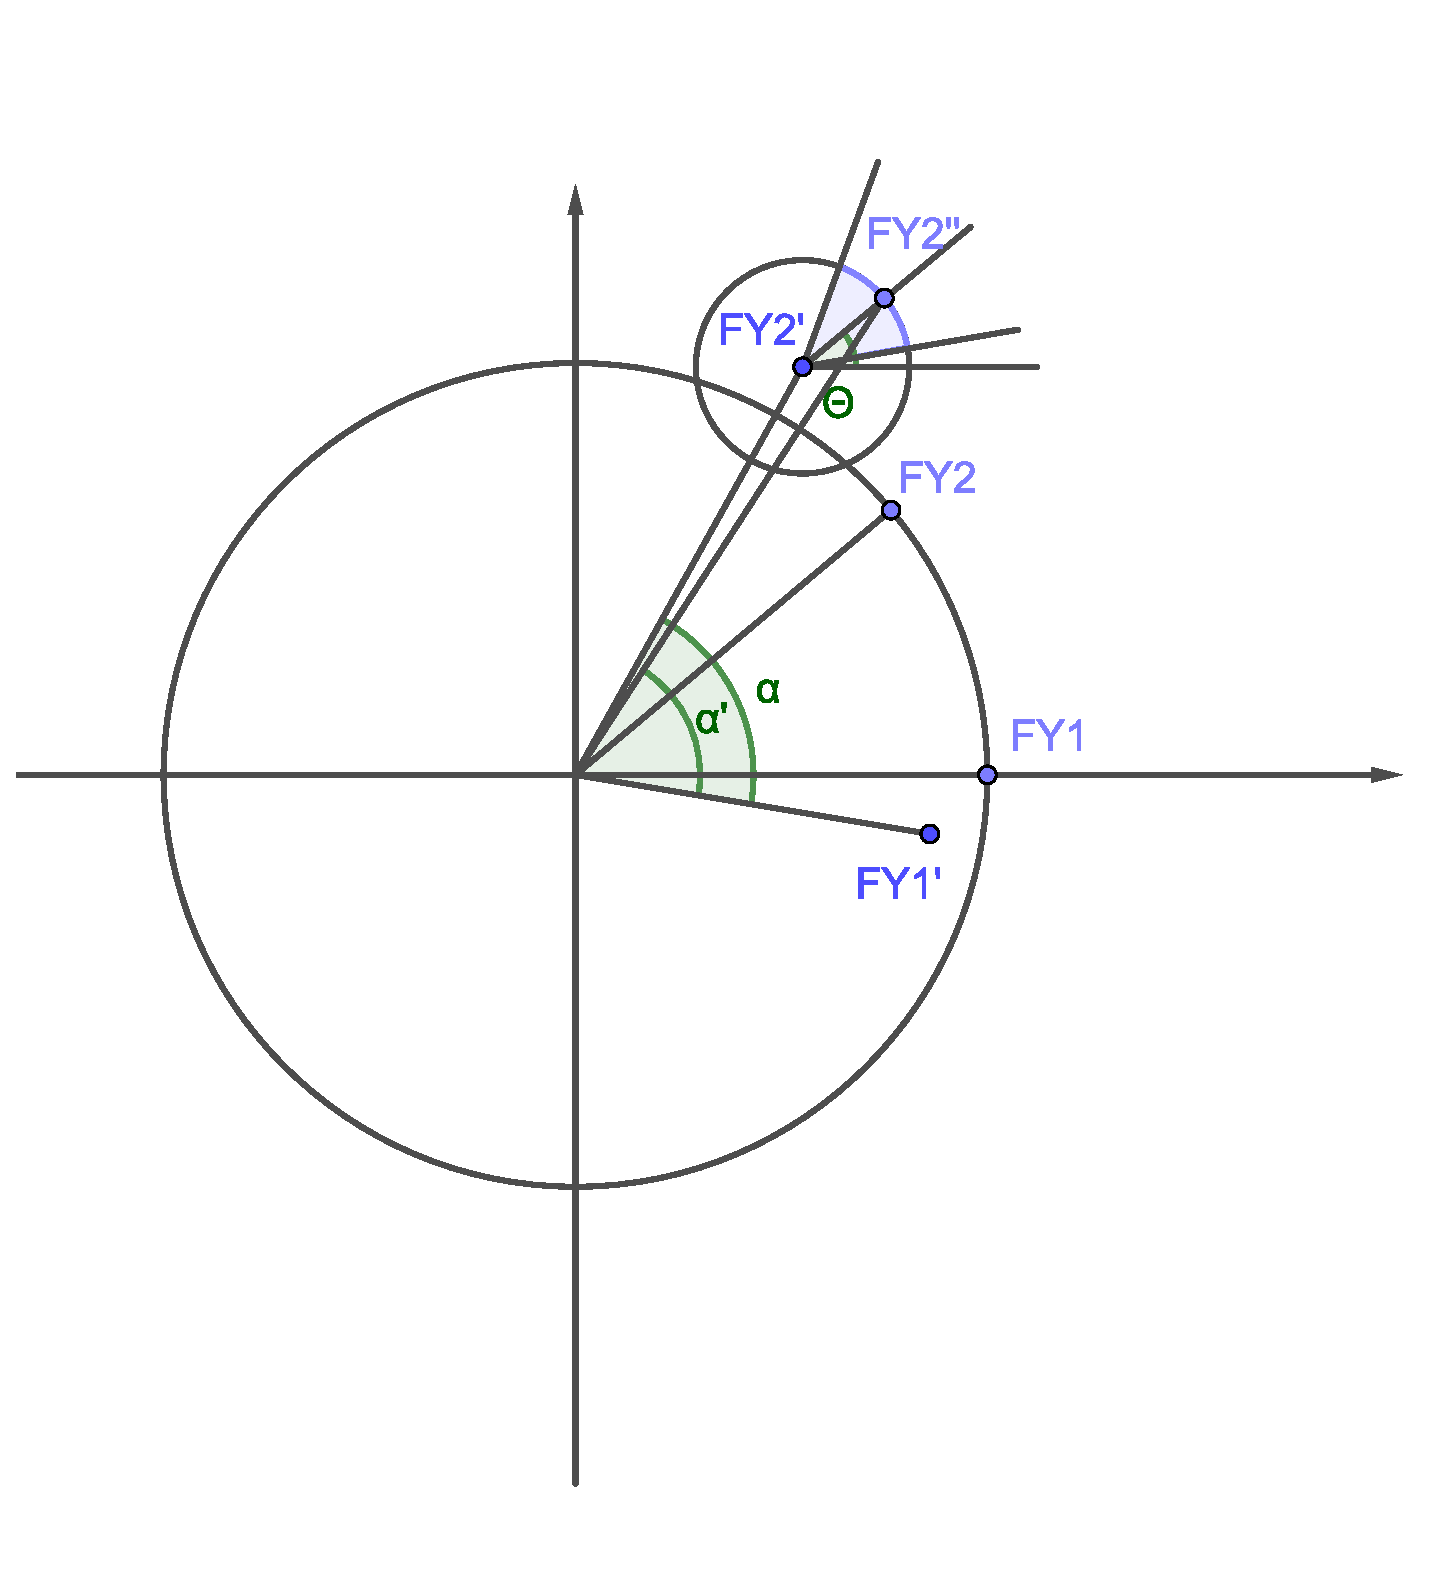
\includegraphics[width=0.55\linewidth]{pic/bisection.eps}
    \caption{二分移动路径法示意图}
    \label{二分移动路径法示意图}
    \end{figure}


    我们可以对其他编号的无人机根据其理想位置确定不同的$\theta$范围,在各自的范围内分别二分移动路径,最终确定各自位置到原点的连线和x轴的夹角大小。
\subsubsection{结果求解}

当二分移动结束后,可以通过前几次移动的方案求出该编号无人机当前所在的位置。位置坐标在极坐标系下表示,极坐标系的极轴与原平面直角坐标系的x轴重合。

a.幅角的计算

设无人机共移动N次到达期望位置,第i次无人机的移动指令为$(\Delta X_i,\Delta Y_i)$,最终状态下无人机在水平方向上移动了$\sum_{i=1}^{N}\Delta X_i$的距离,在竖直方向上移动了$\sum_{i=1}^{N}\Delta Y_i$的距离。

所以,这N次移动等价于从初始点到最终点进行一次移动$(\sum_{i=1}^{N}\Delta X_i,\sum_{i=1}^{N}\Delta Y_i)$。

由于二分法的目的是使最终状态无人机的位置幅角等于初始状态无人机的位置幅角。故幅角计算公式为:

\begin{equation}
  \theta=arctan(\frac{\sum_{i=1}^{N}\Delta Y_i}{\sum_{i=1}^{N}\Delta X_i})
\end{equation}

b.极径的计算

选取相邻两个无人机求解三角形,如图\ref{三角形求解示意图}所示:


\begin{figure}[H]
  \centering
  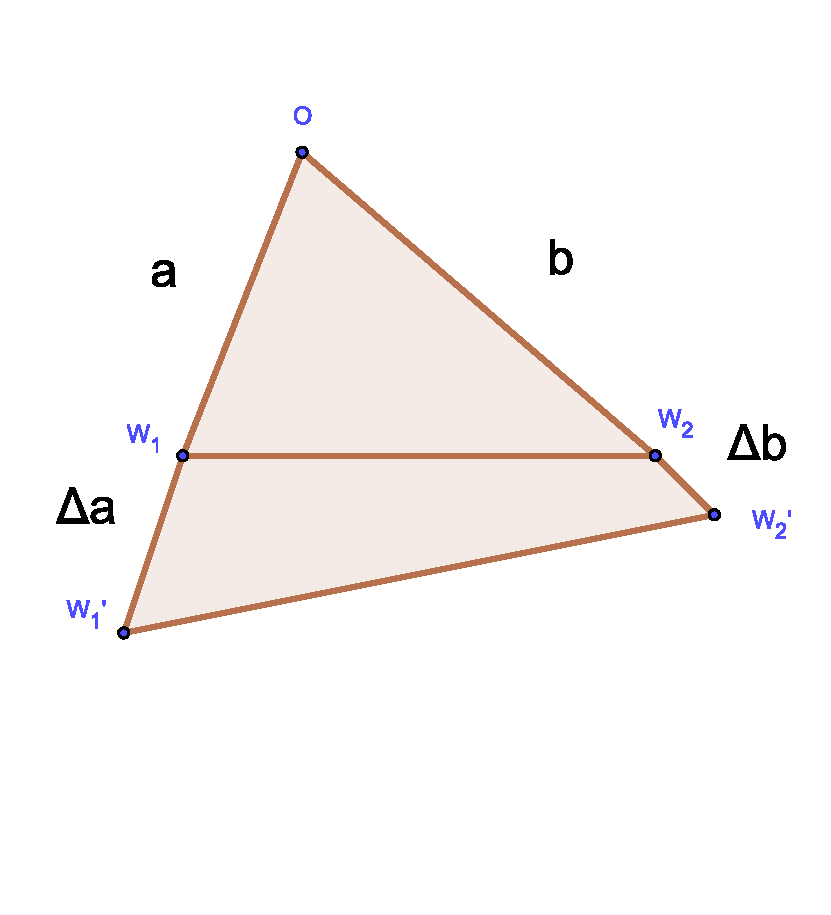
\includegraphics[width=0.45\linewidth]{pic/solution.eps}
  \caption{三角形求解示意图}
  \label{三角形求解示意图}
  \end{figure}



$\Delta OW_1W_2$为两无人机在初始位置时形成的三角形,$\Delta OW_1^{'}W_2^{'}$为两无人机在最终位置时形成的三角形。经过第一轮的信号发射,可以得到方向信息$\alpha_1$,$\beta_1$;经过最终一轮的信号发射,可以得到方向信息$\alpha_2$,$\beta_2$。

其中a为$W_1$无人机在初始时的极径,b为$W_2$无人机在初始时的极径。$\Delta a$为$W_1$无人机最终位置与初始位置的距离,$\Delta b$为$W_2$无人机最终位置与初始位置的距离。

利用正弦定理解三角形可得:

\begin{equation}
  \left\{
            \begin{array}{ll}
              b=\frac{\Delta b-\Delta a}{\frac{sin\alpha_1}{sin\beta_1}-\frac{sin\alpha_2}{sin\beta_2}}\\
              a=\frac{\Delta b-\Delta a}{1-\frac{sin\alpha_2\cdot sin\beta_1}{sin\alpha_1\cdot sin\beta_2}}\\


            \end{array}
          \right.
\end{equation}

其中,
\[
  \Delta a=\sqrt{(\sum_{i=1}^{N}\Delta X_{i,1})^2+(\sum_{i=1}^{N}\Delta Y_{i,1})^2}
\]
\[
  \Delta b=\sqrt{(\sum_{i=1}^{N}\Delta X_{i,2})^2+(\sum_{i=1}^{N}\Delta Y_{i,2})^2}
\]
则$W_1$无人机现在所在的位置$W_1^{'}$的极径为a+$\Delta a$,$W_2$无人机现在所在的位置$W_2^{'}$的极径为b+$\Delta b$。

获得所有无人机在极坐标系上的坐标后,即可将其按照理想位置一步移动到位。
\subsubsection{结果展示}
为使二分法尽可能精确(控制幅角误差在$10^{-6}$左右),我们设定整个流程循环20次,即共经历21轮次信号发射,其中每轮次包含4次不同发射源的信号发射。故至多需要84次不同发射源的信号发射,即可实现有效定位。

题目要求无人机在最终需调整到理想位置,使得9架无人机最终均匀分布在圆周上。本文将理想位置设定为如表1所示的标准坐标。
\subsubsubsection{方案展示}

由于方案中信号发射的次数较多,故完整方案无法在正文中展示,而放于附录中。方案包括每一轮发射源的选择以及各编号无人机的移动距离。

计算发现,累积误差(9个点求解位置与理想位置的距离和)为0.000160328m,说明求解效果良好。

\subsubsubsection{模型的进一步检验}

由于题中所给的初始点的位置相较理想位置的误差较小,故为了对模型进行更好的检验,我们考虑扩大误差观察求解效果。

将误差限扩大到30\%(即极径误差为$\pm 15m $,幅角误差为$\pm 9^{\circ}$)进行模拟。

模拟方法为:在9个理想位置附近各框定30\%的误差区域,每一个误差区域中随机选取一个点作为该区域编号无人机的初始位置。将其作为输入代入求解具体调整方案。

模拟1000000次的试验后,我们发现累积误差均控制在$10^{-3}$m以内,说明在误差较大的情况下也能进行较优的求解,使9个偏移位置点移动到标准位置。

\subsection{问题四的分析解决}
我们尝试将求解问题三的方法推广运用到问题四中。考虑在锥形编队情景下,仍选取一对无人机位置固定不动、形成一条固定的信号边;对其他无人机尝试移动时,寻找控制其与该边夹角不变的移动方向,即可得到其初始位置与坐标轴的方向角。具体实现过程中,仍可沿用三题中所述的二分查找方法,通过在一小段轨迹圆弧中不断尝试来得到所求方向。

\subsubsection{坐标轴的建立与测量基准点无人机的选取} 

建立坐标轴的整体考量与问题三类似:选取FY01作为坐标原点;假定图中机群机头朝向为其前进方向,定为x轴正方向,再以右手螺旋形式建立y轴即可,如图\ref{坐标系建立示意图}所示。验证知在该坐标系中各无人机的位置均能较简洁地表示出来,坐标系建立合理。

\begin{figure}[H]
  \centering
  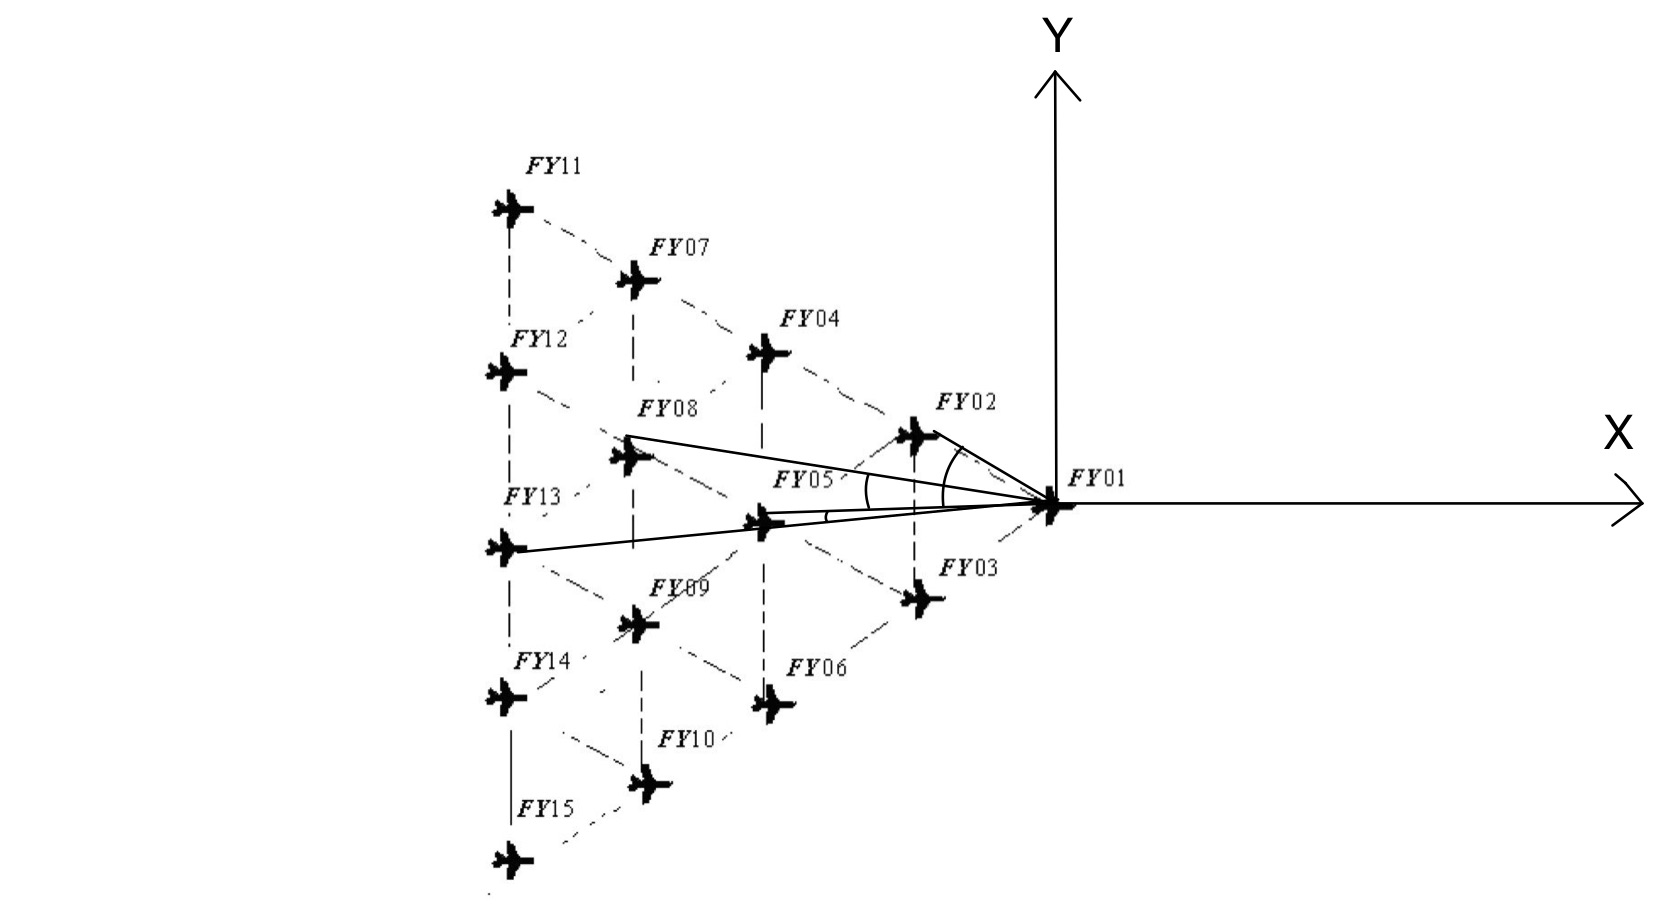
\includegraphics[width=0.55\linewidth]{pic/share.jpg}
  \caption{坐标系建立示意图}
  \label{坐标系建立示意图}
  \end{figure}

首先我们考虑固定FY01作为测量基准点。因为FY01处于编队的顶角位置,其他无人机均在其周围一个较小的角度范围内,能使测量得到的角度在一个大小合理的角度区间。接着我们考虑固定FY05作为另一基准点。因为大部分无人机均对称分布在FY01-FY05轴线两侧,能保证后续二分时大部分点所取的轨迹区间使得其与固定边的夹角单调变化,
即使问题拥有可二分性。

同时初始轮次二分进行各个无人机方位角的测定时,FY13虽不是基准点、但也先固定不动。这是考虑到FY13位于上述选定的FY01-FY05轴线附近,所选取的查找轨迹区间可能穿越轴线,使其丧失了用于二分的角度单调性,不能得到其方向角的真实值。我们将在后续轮次中单独考虑为FY13定位的问题。

\subsubsection{二分移动路径法}
在锥形编队队形下,我们可以通过控制其他无人机到$FY01$的连线与$FY01FY05$这条边的夹角大小,二分确定其他无人机的方向,具体二分方法和问题一的第3小问的方法类似,但由于$FY01$可以作为接收点,我们可以直接得到夹角的角度信息,而不是通过三角形内其他两个角的角度,间接计算夹角。

\subsubsection{结果求解}

由上文阐述的发射信号与移动方案可知,在二分循环中FY01、FY05、FY13均未移动。将15架无人机的当前位置分成三类计算:

(1)FY01编号无人机为测量基准点,假设其初始位置即为标准位置,则其当前位置为原点(0,0);

(2)除FY01、FY05、FY13这三个点外,其余点按第三问中的方式进行求解。其中:

a.幅角计算公式
\[
  \theta=arctan(\frac{\sum_{i=1}^{N}\Delta Y_i}{\sum_{i=1}^{N}\Delta X_i})
\]

b.极径的计算

选取FY01,FY05以及所需求解的点的位置解三角形,即在图\ref{三角形求解示意图}的情况下,令$\Delta b$=0。

故极径的计算公式为:

\begin{equation}
              a=\frac{\Delta a}{\frac{sin\alpha_2\cdot sin\beta_1}{sin\alpha_1\cdot sin\beta_2}-1}\\
\end{equation}

则$W_1$无人机现在所在的位置$W_1^{'}$的极径为a+$\Delta a$。

(3)FY13编号的无人机由于无法用二分法求解的限制,需要借助其他手段进行位置求解。


再发射一次信号,分别为FY01(O),FY13(Q)以及在X轴上方的无人机(例如FY02(P)),得到相应的方向信息$\angle POQ$。

a.幅角的计算

由于P点与X轴的夹角已知,P点与Q点的夹角已知,且Q点在P点的逆时针方向,故幅角计算公式为:

\begin{equation}
  \theta_Q=\theta_P-\angle POQ
\end{equation}

b.极径的计算

由于P点与原点间的距离已知,故应用正弦定理可知Q点的极径:

\[
  OQ=OP\times \frac{sin \angle OPQ}{sin\angle OQP}
\]

获得所有无人机在极坐标系上的坐标后,即可将其按照理想位置一步移动到位。

\subsubsection{结论说明}

当需要定位的无人机偏差过大时,如$FY08$偏差到了$FY01-FY05$连线下方,则会使其丧失可二分性,可能导致求解失败。当偏差较小时,则可以在共$20$轮询问和调整后,将每个无人机的角度偏差降低到$10^{-5}$以内。

\section{模型的评价与推广}
\subsection{模型的优点}
    \begin{itemize}
      \item 定位精度高,问题一(1)的定位误差可基本控制在$10^{-8}m$内,问题一(2)(3)的定位误差和累积误差可基本控制在$10^{-4}m$内。
      \item 使用无人机接收到的角度信息验证定位准确性,可以在实际应用时进行检验,不需要得知真实坐标,适用性强,且在计算机模拟时检验结果和用真实坐标的检验结果相同,正确性高。
      \item 投票机制让定位错误率大大下降,同时尽量使用了少的发射无人机进行定位,且投票机制衍生出的二轮投票机制可以进一步延伸,得到使用三架甚至更多未知编号的发射无人机进行定位的多轮投票模型,进一步提高定位精度和正确率。
    \end{itemize}
\subsection{模型的缺点}
    \begin{itemize}
      \item 当需要定位的无人机距离其理想位置偏差较大时,模型可能出现定位错误的情况,此时可以考虑加入更多发射源。
      \item 基准无人机需要处理的角度信息远多于其他无人机,对其计算性能和精度要求较高。
      \item 在投票模型中计算误差圆对应的角度范围时使用了较为方便实现的蒙特卡洛方法,精度较低且复杂度较高,可以考虑改用论文提到的计算几何相关的计算方法。
      \item 在最后一次调整到接近理想位置之前,在前期二分调整时,各无人机可能会先远离理想位置。
    \end{itemize}
\subsection{模型的推广}
    问题一(1)中的定位模型可以推广到用平面上任意3个已知位置的发射源及接收点得到的角度信息来定位一个已知大致位置的接收点,不必局限在圆周附近进行定位。

    问题一(3)和问题二中先二分确定角度,再解三角形确定距离以定位每个无人机和基准无人机的相对位置的思路也可以拓展到其他编队队形的调整上。

    

\begin{thebibliography}{100}%此处数字为最多可添加的参考文献数量
  \bibitem{article1} 赵骁飞. 单站纯方位无源探测定位的若干技术的研究[D].上海交通大学,2007.
\end{thebibliography}







  


















\end{document}